% -*- Mode:TeX -*-

%% The documentclass options along with the pagestyle can be used to generate
%% a technical report, a draft copy, or a regular thesis.  You may need to
%% re-specify the pagestyle after you \include  cover.tex.  For more
%% information, see the first few lines of sk-thesis.cls. 

% DRAFT MODE uses simpler front page, without dedication, acknowledgements, uses a footer sying draft.
%\documentclass[12pt,a4paper,vi,twoside,leftblank]{sk-thesis}
\documentclass[12pt,a4paper,vi,draft]{sk-thesis}
%\documentclass[12pt,a4paper,vi]{sk-thesis}
\usepackage[utf8]{inputenc}
\usepackage{geometry}
\geometry{a4paper, right=30mm, bottom=30mm, left=30mm, top=30mm}

\usepackage{ifdraft}
\usepackage{graphicx}
\setkeys{Gin}{draft=false} % disable hiding graphics in draft mode
\usepackage[table]{xcolor}
\usepackage{multicol, multirow}
\usepackage{amsmath, amssymb}
\usepackage{cmap}
\usepackage[T1]{fontenc}
\setlength {\marginparwidth }{2.5cm} 
\usepackage[obeyDraft]{todonotes}
\usepackage{booktabs, siunitx}
\usepackage[breaklinks=true]{hyperref}
\usepackage{natbib, breakcites}
\usepackage{bibentry}
\usepackage{doi}
\definecolor{navyblue}{rgb}{0.0, 0.0, 0.5}
%\definecolor{royalblue}{rgb}{0.06, 0.11, 0.42}
\hypersetup{
  final,
  colorlinks=true,
  urlcolor=navyblue,
  citecolor=navyblue,
  linkcolor=navyblue
}
\usepackage{cleveref}
\crefformat{footnote}{#2\footnotemark[#1]#3}
\usepackage{catoptions}
\makeatletter
%\def\figureautorefname{figure}
%\def\tableautorefname{table}
\def\Autoref#1{%
  \begingroup
  \edef\reserved@a{\cpttrimspaces{#1}}%
  \ifcsndefTF{r@#1}{%
    \xaftercsname{\expandafter\testreftype\@fourthoffive}
      {r@\reserved@a}.\\{#1}%
  }{%
    \ref{#1}%
  }%
  \endgroup
}
\def\testreftype#1.#2\\#3{%
  \ifcsndefTF{#1autorefname}{%
    \def\reserved@a##1##2\@nil{%
      \uppercase{\def\ref@name{##1}}%
      \csn@edef{#1autorefname}{\ref@name##2}%
      \autoref{#3}%
    }%
    \reserved@a#1\@nil
  }{%
    \autoref{#3}%
  }%
}
\makeatother
\usepackage{textcomp}
\usepackage{fancyhdr}
\newcommand{\changefont}{%
    \fontsize{10}{10}\selectfont
}
\fancyhf{}
%\fancyhead[LE]{\slshape \rightmark} %section
%\fancyhead[RE]{}
%\fancyhead[RO]{\slshape \leftmark} % chapter
%\fancyhead[LO]{}
\fancyhead[LE,RO]{\changefont \slshape \nouppercase{\rightmark}} %section
\fancyhead[RE,LO]{\changefont \slshape \nouppercase{\leftmark}} %chapter
\fancyfoot[C]{\thepage} %footer
\usepackage{datetime}
\usepackage[automake,toc]{glossaries}
\glsenablehyper
\makeglossaries
%\usepackage{comment}
\usepackage{subcaption}
\usepackage{tabularx, lscape, rotating}
\usepackage[most]{tcolorbox}
\newtcolorbox{myframe}[1][]{
  enhanced,
  top=12pt,bottom=12pt,left=16pt,right=16pt,
  arc=0pt,
  outer arc=0pt,
  colback=white,
  boxrule=1pt,
  #1
}

%%%%%%%%%%%% EPIGRAPH
\usepackage{epigraph}
%\setlength{\beforeepigraphskip}{1.0\baselineskip}
\setlength{\epigraphrule}{0pt}
\setlength{\epigraphwidth}{.4\textwidth}
%\setlength{\afterepigraphskip}{.25\baselineskip}
\renewcommand{\textflush}{flushepinormal}
    
\ifdraft{
    %% LIMIT CHAPTERS
    \includeonly{
        prelude,
        contents,
        chapters/01_introduction,
        chapters/02_literature_review,
        chapters/03_materials_and_methods.tex,
        chapters/04_results,
        chapters/05_conclusion,
        glossary,
        bibliography,
%        chapters/appendix-a
    }
}{
}

\begin{document}

\ifdraft{
    %%%%%%%%%%% HEADERS AND FOOTERS
    \fancypagestyle{plain}{%
      \fancyhf{}%
      \renewcommand{\headrulewidth}{0pt}% Line at the header invisible
      \fancyfoot[L]{\changefont PhD Thesis - Student Name} % DRAFT ONLY
      \fancyfoot[C]{\thepage}% \changefont 
      \fancyfoot[R]{\changefont \textbf{DRAFT} \today} % DRAFT ONLY
    }
    \fancyfoot[L]{\changefont PhD Thesis - Student Name} % DRAFT ONLY
    \fancyfoot[R]{\changefont \textbf{DRAFT} \today} % DRAFT ONLY
    \pagestyle{fancy}
    
    %% SIMPLE TITLE PAGE
    \chapter*{A deep learning framework for mixed dense forests parameter estimation at individual tree scale}

\begin{center}
\Large{
\textsc{PhD Thesis (Final Draft) \\ Ivan Dubrovin \\ }
}

\today\ \currenttime
\end{center}

\clearpage

\section*{Abstract}
In short this is the content of my work...

\section*{Publications}
\subsection*{Main author}
\nobibliography*
\begin{enumerate}
    \item \bibentry{dubrovinRemoteSensingEvidence2022}
    \item \bibentry{dubrovinExplorationPropertiesPoint2024}
    \item \bibentry{dubrovinOpenDatasetIndividual2024}
\end{enumerate}

\listoftodos
\clearpage
}{
    %% FULL TITLE PAGE
    % -*-latex-*-
% NOTE:
% These templates make an effort to conform to the Skoltech Thesis specifications,
% however the specifications can change.  We recommend that you verify the
% layout of your title page with your thesis advisor and the Education department 
% before printing your final copy.
\title{A deep learning framework for mixed dense forests parameter estimation at individual tree scale}

\author{Ivan Dubrovin}
% If you wish to list your previous degrees on the cover page, use the 
% previous degrees command:
%       \prevdegrees{MSc, University of Salzburg (2007)}
% You can use the \\ command to list multiple previous degrees
%       \prevdegrees{B.S., University of California (1978) \\
%                    S.M., Massachusetts Institute of Technology (1981)}
\department{Center for Digital Engineering}

\degree{Doctoral Program in Engineering Systems}

\degreemonth{December}
\degreeyear{2024}
\thesisdate{November 2024}

%% By default, the thesis will be copyrighted to MIT.  If you need to copyright
%% the thesis to yourself, just specify the `vi' documentclass option.  If for
%% some reason you want to exactly specify the copyright notice text, you can
%% use the \copyrightnoticetext command.  
%\copyrightnoticetext{\copyright \@author \@degreeyear}

% If there is more than one supervisor, use the \supervisor command
% once for each.
\supervisor{Clement Fortin}{Professor}

% This is the department committee chairman, not the thesis committee
% chairman.  You should replace this with your Department's Committee
% Chairman.
%\chairman{Name}{Title}

% Make the titlepage based on the above information.  If you need
% something special and can't use the standard form, you can specify
% the exact text of the titlepage yourself.  Put it in a titlepage
% environment and leave blank lines where you want vertical space.
% The spaces will be adjusted to fill the entire page.  The dotted
% lines for the signatures are made with the \signature command.
\maketitle

% The abstractpage environment sets up everything on the page except
% the text itself.  The title and other header material are put at the
% top of the page, and the supervisors are listed at the bottom.  A
% new page is begun both before and after.  Of course, an abstract may
% be more than one page itself.  If you need more control over the
% format of the page, you can use the abstract environment, which puts
% the word "Abstract" at the beginning and single spaces its text.

%% You can either \input (*not* \include) your abstract file, or you can put
%% the text of the abstract directly between the \begin{abstractpage} and
%% \end{abstractpage} commands.

% First copy: start a new page, and save the page number.
\cleardoublepage
% Uncomment the next line if you do NOT want a page number on your
% abstract and acknowledgments pages.
% \pagestyle{empty}
\setcounter{savepage}{\thepage}
\begin{abstractpage}
In short this is the content of my work...
\end{abstractpage}


\clearpage
\section*{Publications}
\subsection*{Main author}
\nobibliography*
\begin{enumerate}
    \item \bibentry{dubrovinRemoteSensingEvidence2022}
    \item \bibentry{dubrovinExplorationPropertiesPoint2024}
    \item \bibentry{dubrovinOpenDatasetIndividual2024}
\end{enumerate}

\cleardoublepage

\begin{dedication}
Dedicated to my parents.
\end{dedication}

\section*{Acknowledgments}

Work in progress. My supervisor, professor Clement Fortin. My previous super- visor, professor Anton Ivanov. Alexander Kedrov and Albert Vasiliev from Space Technologies and Services Center, Ltd. My beautiful patient wife.

    
    %%%%%%%%%%% HEADERS AND FOOTERS
    \fancypagestyle{plain}{%
      \fancyhf{}%
      \renewcommand{\headrulewidth}{0pt}% Line at the header invisible
      \fancyfoot[C]{\thepage}%
    }
    \pagestyle{fancy}
}
  % -*- Mode:TeX -*-
%% This file simply contains the commands that actually generate the table of
%% contents and lists of figures and tables.  You can omit any or all of
%% these files by simply taking out the appropriate command.  For more
%% information on these files, see appendix C.3.3 of the LaTeX manual.

\begin{singlespace}
    \tableofcontents
\end{singlespace}
\newpage
%\ifdraft{
%}{
\begin{singlespace}
    \listoffigures
\end{singlespace}
\newpage
\begin{singlespace}
    \listoftables
\end{singlespace}
%}
\chapter{Introduction}\label{cap:introduction}

This chapter aims to give a general introduction to the research project and put it into wide scientific and societal context.
It defines the main research question and the hypothesis, and gives a high-level overview of the proposed framework.
It also provides the links to the original datasets and the code.

\section{Context}
Forests are a crucial part of the global ecosystem, both environmentally and economically.
They cover a third of the land area, contain over 80\% of terrestrial biodiversity, and somewhere around one-third of humanity depends on forests and forest products for their livelihoods [\citet{aertsForestRestorationBiodiversity2011}; \citet{StateWorldsForests2020}].
Forests are an essential renewable natural resource and a huge, dynamic part of the global carbon cycle.
Figure~\ref{fig-forest-coverage} offers a map of the global tree coverage based on data from \citet{hansenHighResolutionGlobalMaps2013} to highlight the extent of forests on the planet.
Responsible management of forests allows using the resources efficiently and sustainably, preserving the biodiversity, and regulating atmospheric $CO_2$, which is becoming especially important as the anthropogenic climate change is ongoing and accelerating [\citet{faheyForestCarbonStorage2010}; \citet{forsterIndicatorsGlobalClimate2024}].
This drives the need for accurate, detailed, up-to-date information about various forest attributes such as distributions of tree species, average heights and ages of trees, estimates of trunk diameter, timber volume, and above ground biomass, and others.

The traditional manual forest inventories that rely on people going out into the forest to count and measure trees are extremely labor-intensive and time-consuming, which makes them infeasible to cover extensive areas with sufficient detail, speed, and frequency \citep{burleyEncyclopediaForestSciences2004}.
This is especially relevant in countries where massive areas are covered by forests, such as Russia, Brazil, Canada, USA, and China, which are the top five countries for forest area according to \citet{GlobalForestResources2020}.
For that reason, various remote sensing techniques are widely used to extend and extrapolate the traditional forest inventories.
All sorts of data, from satellite and aerial imagery to very detailed terrestrial \gls{lidar} surveys, are used in all sorts of applications that require mapping forest attributes.
Some such applications are mentioned in the next chapter dedicated to reviewing the literature.

\begin{figure}
\centering{
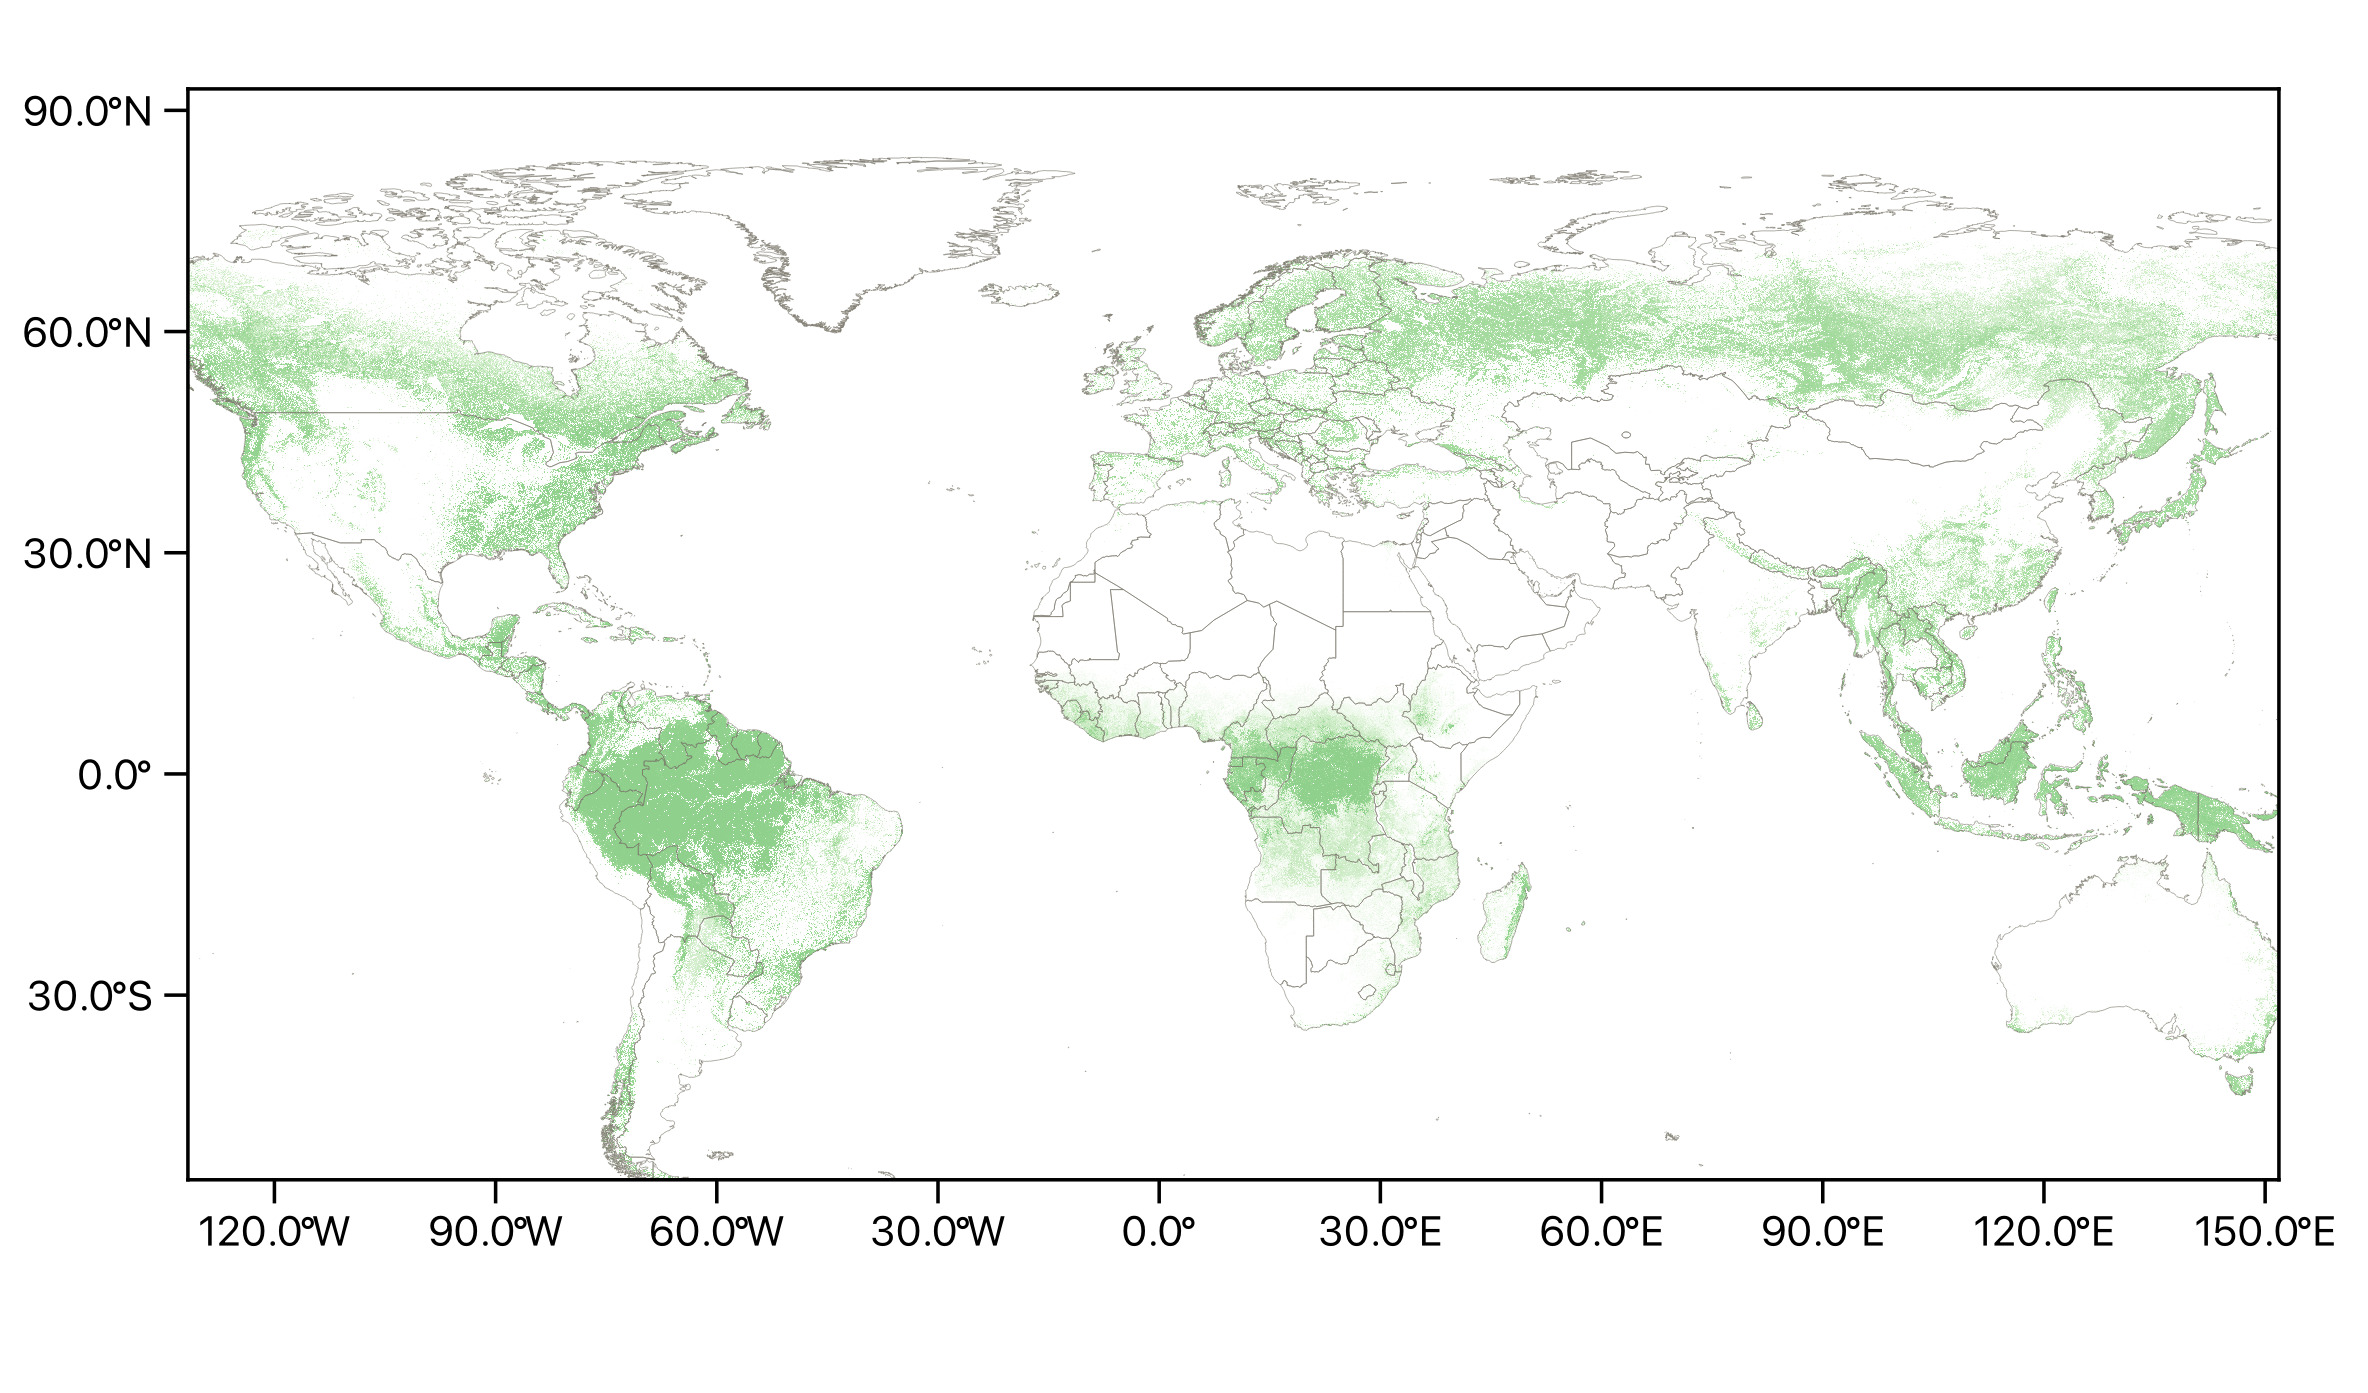
\includegraphics[width=\textwidth]{../images/global-forest-cover.jpg}
}
\caption[Global tree cover map]{\label{fig-forest-coverage}Global tree cover for 2010. Area occupied by tree canopies relative to the total area of the pixel. Data from \citet{hansenHighResolutionGlobalMaps2013}
}
\end{figure}

Many national space agencies even provide open access to satellite data that can be used for mapping forests.
European Space Agency offers free and open access\footnote{Although the access is not open for everyone equally, as I have observed silent bans of the accounts connecting from Russian IP addresses without any response to support inquires in the previous platform, and an outright IP ban in the current one.} to the Sentinel missions through its \href{https://dataspace.copernicus.eu/}{Copernicus Data Space Ecosystem} platform, including C-band SAR data from Sentinel-1 and medium-resolution multispectral data from Sentinel-2, both with global coverage.
They also have an upcoming P-band SAR mission called BIOMASS, designed specifically to study global forest biomass and carbon cycles \citep{queganEuropeanSpaceAgency2019}, which further indicates the growing importance and interest in the topic of forest mapping.
\gls{nasa} provides free access to an abundance of satellite data through its \href{https://www.earthdata.nasa.gov/}{Earthdata platform}, Landsat mission with the \gls{oli} instrument and Terra mission with \gls{modis} instrument being the most relevant for forest mapping applications.
The Indian Space Research Organisation, Brazilian National Institute for Space Research, National Space Research and Development Agency of Nigeria all offer free satellite data that can be used for this purpose.
\gls{nasa} and the \gls{isro} also have a joint upcoming mission called NISAR with two fully-polarimetric SAR sensors at L-band and S-band \citep{kelloggNASAISROSyntheticAperture2020}, which will benefit forestry applications greatly.

The open satellite data is an essential tool for wide-area studies, but it usually has coarse resolution (tens to hundreds of meters per pixel), which limits the achievable accuracy and level of detail.
It also offers no ability to control the observation parameters, as they are fixed by the instrument configuration and orbit parameters, both of which are outside the data consumer control.
Higher resolution data with a limited ability to control the acquisition parameters is available commercially, but the prices are steep.
Aerial observations with sensors mounted on planes or helicopters are both more controllable and cheaper alternatives, although still expensive and sill limited in the flexibility of the control of acquisition parameters.
A much more affordable and controllable alternative is \gls{uav}-based observation.
It allows for fine-grained control and on the fly adjustment of many important parameters such as flight height, flight path overlap, combination of used sensors, and so on.

The most common way to use \gls{uav} remote sensing, be it \gls{lidar}, multispectral, hyperspectral, or other data modalities, for mapping forest attributes in industry is what is known in the \gls{lidar} community as the area-based approach, described in detail in Section~\ref{sec-area-based-approach}.
It is based on extrapolating measurements from ground plots made in traditional inventories by aggregating remote sensing data to the grid with cell area of a ground plot, which results in coarse resolution maps.
It is easy to use, but its results are often not detailed enough when working on smaller scales.
However, modern sensors and processing techniques allow not aggregating at all and instead working on the level of individual trees, which is as detailed as it can possibly get, allowing for any level of aggregation for downstream tasks.
This requires robust algorithms that allow detecting individual trees in dense multimodal data.
This is relatively\footnote{The word relatively does a lot of heavy lifting here, as the problem is by no means easy on its own and takes a lot of effort from many researchers to continue to make progress on.
} easy in urban environments, manually planted and managed forest stands, or forests that are either sparse or predominantly coniferous, where the structure of the canopy is easy to interpret.
In some such environments, state-of-the-art results can be achieved by simple local maxima detection algorithms, that rely on the assumption that a tree can be detected by finding peaks on of canopies because they correspond to tree tops.
Forest that are mixed and dense, which are a huge part of forests in countries mentioned earlier, are much harder to work with and are a very active area of research for developing methods of detection of individual trees.
The canopies in such forests are very complex, especially because the top of the crowns of deciduous tree species often do not have a single pronounced height maximum, and crowns of nearby trees often overlap.

The framework described in this thesis focuses on fusion of two remote sensing data sources, \gls{uav} \gls{lidar} point clouds and \gls{uav} \gls{rgb} orthophotos, to detect individual trees in dense mixed forests and predict required attributes for each tree individually, producing the most detailed maps possible.
The choice of data sources is driven by their complementary nature, which I believe is key for semantically parsing such complex environments.
\gls{lidar} is an active sensor, which means it does not depend on external conditions such as lighting.
Cloud and terrain shadows, incidence angles, and weather conditions do not affect \gls{lidar} surveys.
Moreover, \gls{lidar} provides 3D vertical structural information about the forest, as laser pulses penetrate the canopy and reach both the undergrowth and the ground.
This structural information is essential for understanding complex environments like dense forests.
High-resolution \gls{rgb} imagery does depend on the illumination conditions, but is still an invaluable tool, as it offers detailed data with fixed resolution, continuous coverage of surfaces, unlike the discrete representation of laser scanning, and captures many fine details and textures.
It can also benefit from a huge variety of well-established tools and processing techniques from the field of computer vision.
Neither of these data sources on their own is enough to reliably and with sufficient robustness separate individual trees in dense mixed forests, and the key to success lies in their fusion.

\section{Research question and hypothesis}\label{sec-research-question}

The main research question could be formulated as follows: "How to reduce effort and cost required for detailed inventories of dense mixed forests without losing accuracy?"
The main hypothesis is then: "An accurate and detailed inventory with reduced effort and cost can be achieved through fusion of \gls{uav} \gls{lidar} and \gls{rgb} data using machine learning".
The benchmarks to measure against are both the traditional manual forest inventory and the widely used area-based approach.

Cost and effort are closely connected, as any effort is in the end converted to cost.
Still, it often makes sense to separate the two to highlight the nature of the effects the proposed system should have.
The cost reduction was partly addressed in the previous section during the discussion of the platform of choice: \gls{uav}-based remote sensing offers a great balance of upfront cost, effort to operate, and versatility in observation parameters.
The effort reduction comes from greatly decreasing the amount of field inventory data required when using the proposed system, from the relative ease of collection of remote sensing data compared to alternatives, and from relative ease of tuning the system to operate in new areas.

\section{Overview of the framework}

The proposed framework described in this thesis consist of a neural-network based tree segmentation in \gls{uav} \gls{lidar} point clouds enhanced with \gls{rgb} orthophoto-based features and processing the segments with a collection of specialized classic machine learning models that predict the parameters of interest for each detected tree.
The tree segmentation model is trained on synthetic forest patches constructed from a dataset of point clouds of individual trees extracted manually from a large \gls{uav} \gls{lidar} survey, heavily relying on augmentations to make the synthetic forest closer to real forest.
The parameter prediction classification and regression models are trained on the same dataset of individual trees using a collection of widely used manual point cloud features.
Figure~\ref{fig-framework-apply} is a schematic representation of the framework, showing the required inputs in red, processing steps in yellow, and artifacts in cyan.
The field inventory is phased out, but it is still required, as application of any framework requires quality assessment and validation.

\begin{figure}
\centering{
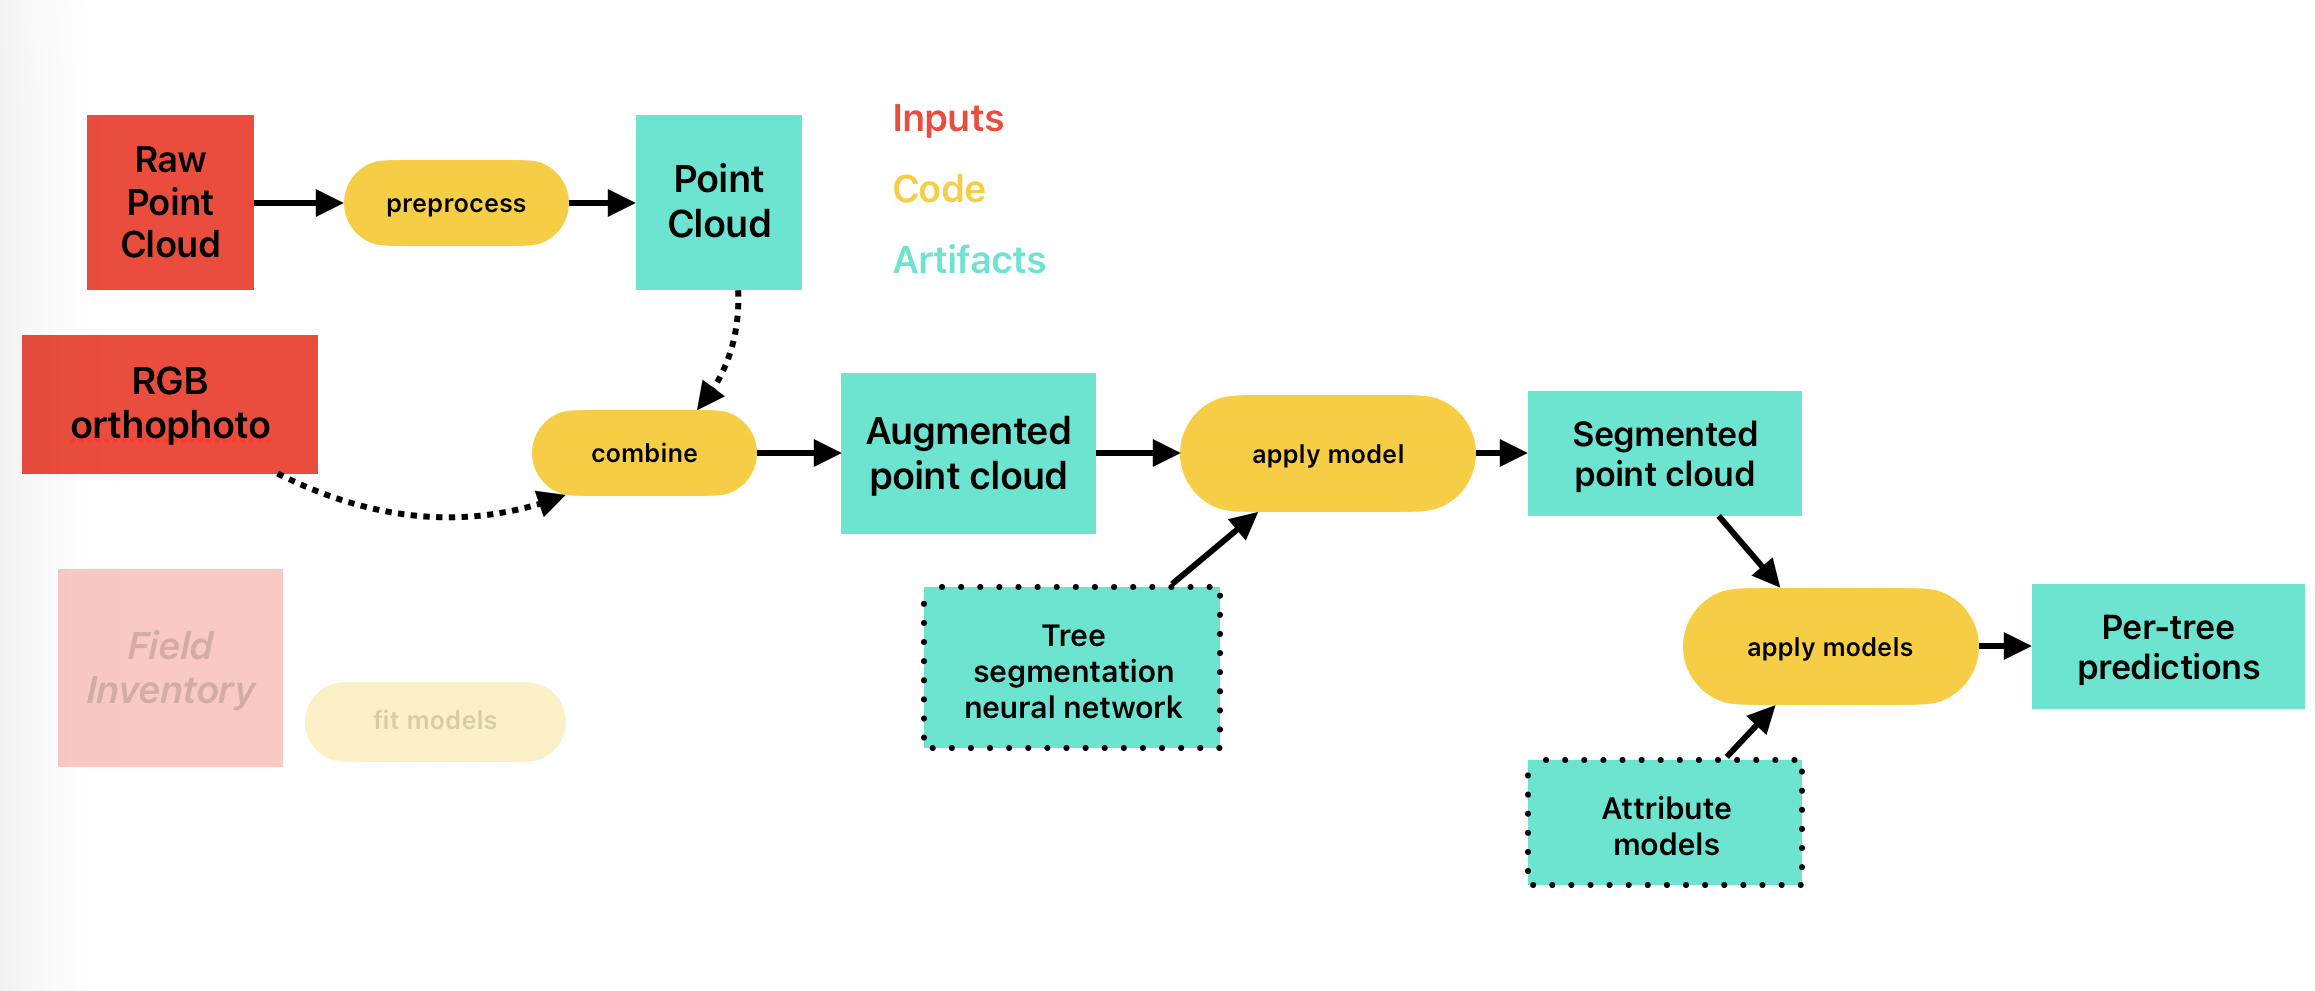
\includegraphics[width=\textwidth]{../images/framework_application_schematic.jpg}
}
\caption[Schematic representation of the framework: application]{\label{fig-framework-apply}The schematic representation of the
framework in the application stage.}
\end{figure}

Figure~\ref{fig-framework-prepare} is a schematic of the preparation step for the framework.
Each individual node is described in detail in Chapter~\ref{cap:materials}.


\begin{figure}
\centering{
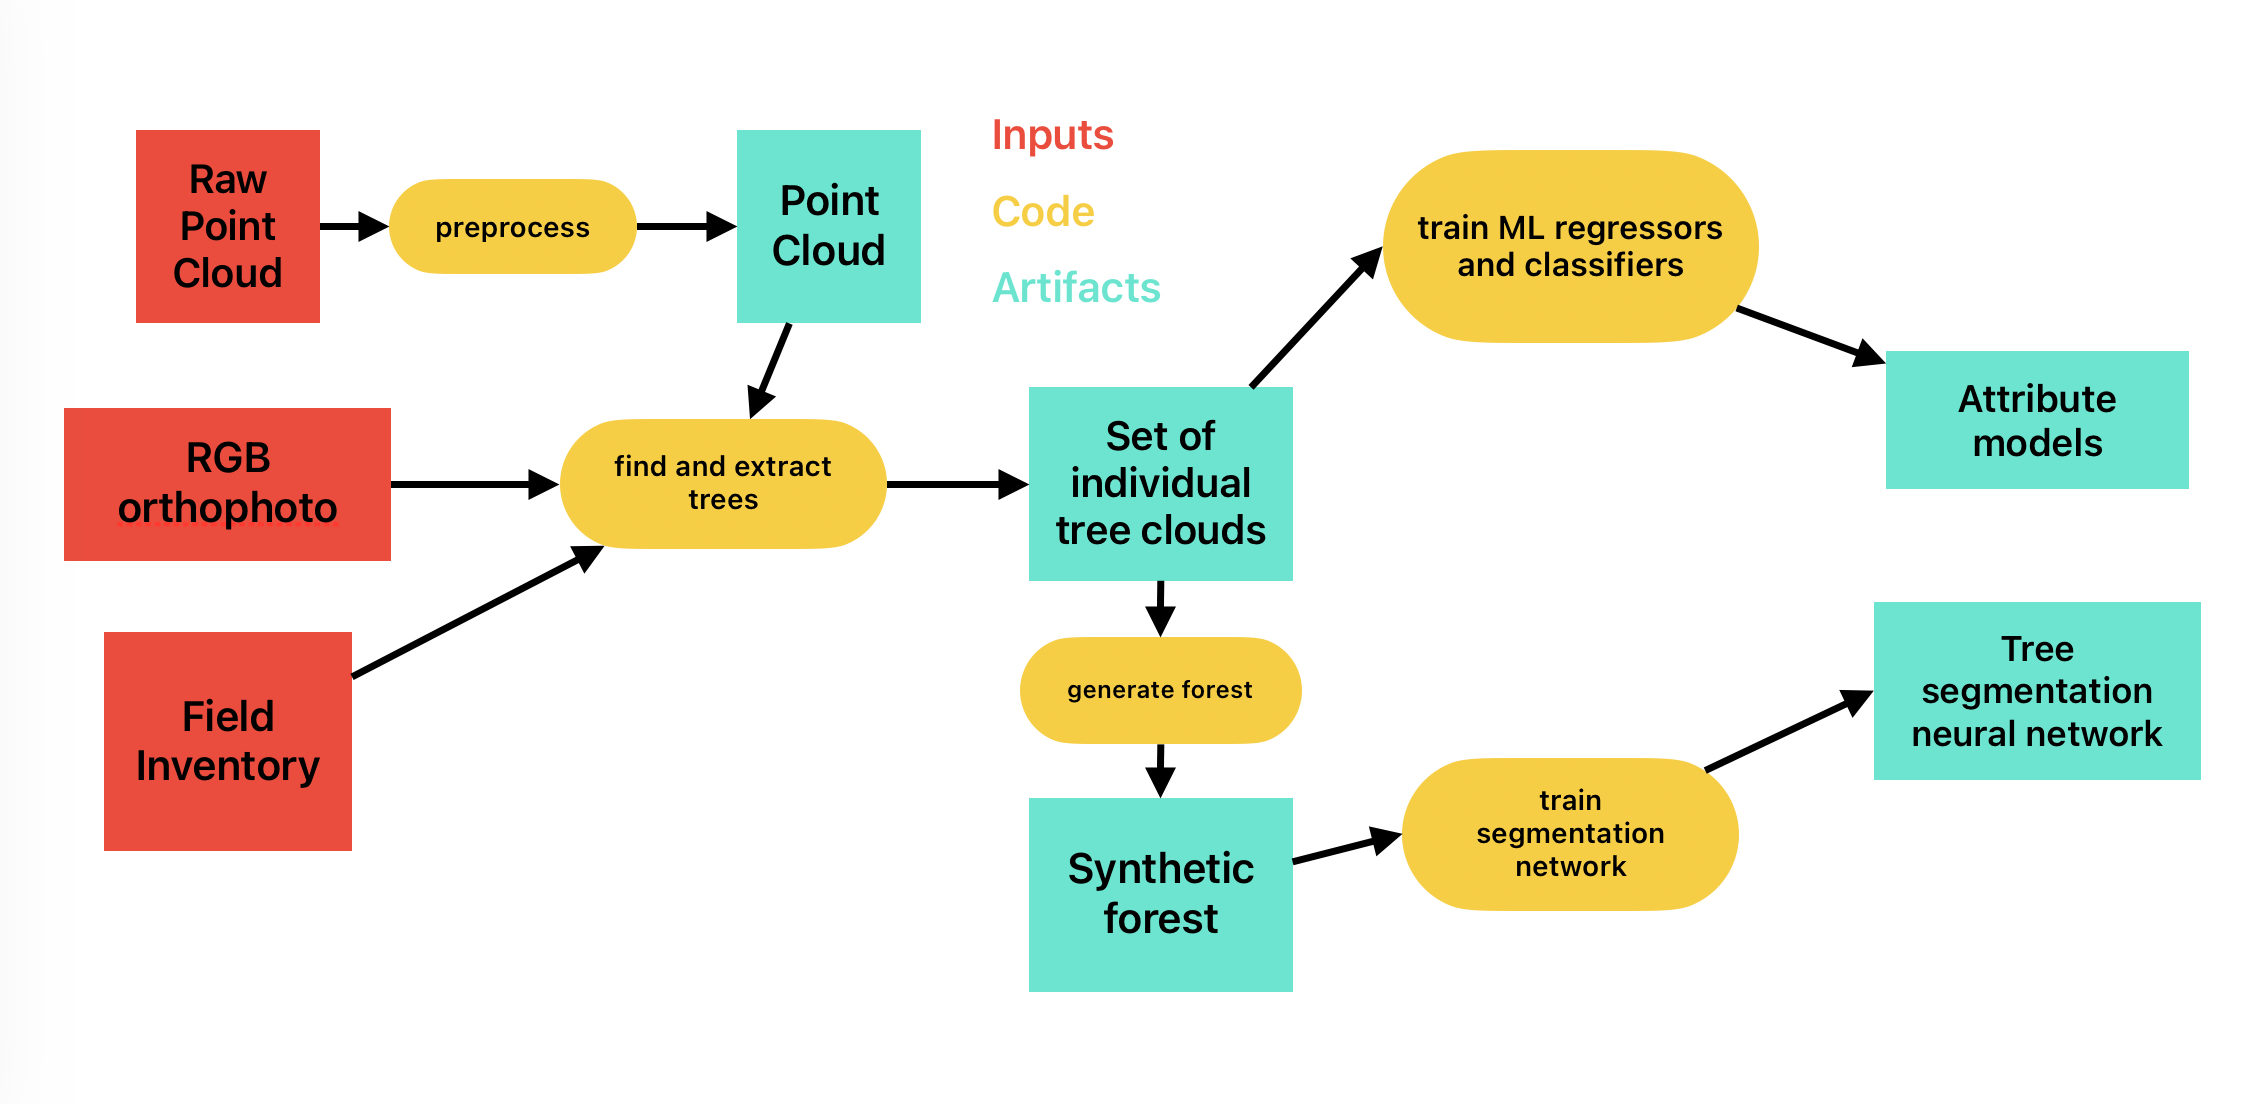
\includegraphics[width=\textwidth]{../images/framework_preparation_schematic.jpg}
}
\caption[Schematic representation of the framework: preparation]{\label{fig-framework-prepare}The schematic representation of
the framework in the preparation stage.}
\end{figure}

\section{Thesis Structure}

\begin{description}
    \item[\Autoref{cap:introduction} - Introduction]
The Introduction chapter aims to give a general introduction to the research project and put it into wide scientific and societal context.
It defines the main research question and the hypothesis, and gives a high-level overview of the proposed framework.
It also provides the links to the original datasets and the code.

    \item[\Autoref{cap:literature} - Literature Review]
The Literature Review chapter aims to give an overview of the scientific literature on topics most relevant to the project.
Its main goals are to provide the reader with context for the research described in the thesis, provide references for in-depth materials on topics that are out of scope of this work, and to highlight the research gap that the work tries to address.

	\item[\Autoref{cap:materials} - Materials and methods]
The Materials and Methods chapter describes in detail the datasets, methods and methodological choices used in the proposed framework.
Its aim is to make the work reproducible and to explain the methodological choices made.

	\item[\Autoref{cap:results} - Results]
The Results chapter describes the results of each stage of the framework preparation and the validation approach used to verify its applicability and effectiveness on realistic data.

    \item[\Autoref{cap:conclusion} - Conclusion]
The Conclusion chapter offers a brief summary of the thesis as a whole, potential perspectives for further improvement of the proposed framework, and some concluding thoughts.

\end{description}

\section{Data and code availability}

Original datasets described in the thesis are openly available on Kaggle \href{https://www.kaggle.com/datasets/sentinel3734/tree-detection-lidar-rgb}{here} and \href{https://www.kaggle.com/datasets/sentinel3734/uav-point-clouds-of-individual-trees}{here}.
All the code used for the project is available on GitHub at \href{https://github.com/iod-ine/phd}{iod-ine/phd}.
An HTML version of this thesis is hosted through GitHub Pages and is available \href{https://iod-ine.github.io/thesis}{here}.
The thesis document was developed using Quarto \cite{Allaire_Quarto_2024} using the literate programming approach \cite{knuth84}, and a link to an HTML version hosted through GitHub Pages is available in the repository.
The deep learning part is implemented using PyTorch \cite{Ansel_PyTorch_2_Faster_2024}, PyTorch Geometric \cite{Fey_Fast_Graph_Representation_2019}, and PyTorch Lightning \cite{Falcon_PyTorch_Lightning_2019}, with experiment tracking using MLflow.
Classic machine learning models implementations are from scikit-learn \cite{scikit-learn}.
NumPy \cite{2020NumPy-Array}, SciPy \cite{2020SciPy-NMeth}, pandas \cite{The_pandas_development_team_pandas-dev_pandas_Pandas}, scikit-image \cite{van_der_Walt_scikit-image_image_processing_2014} libraries are used for processing the data.
ratserio \cite{gillies_2019}, geopandas, laspy, lazrs libraries are used for working with geospatial data formats.
matplotlib \cite{Hunter_Matplotlib_A_2D_2007} and seaborn \cite{waskomSeabornStatisticalData2021} libraries are used for visualization.

\chapter{Literature review}\label{cap:literature}

This chapter provides an overview of the current state of literature on a variety of subjects related to the thesis.
Its main goals are to provide the reader with context for the research described here and to highlight the research gap that the work tries to address.
Where appropriate, references for in-depth materials on topics that are out of scope of this work are provided.

\section{Remote sensing for forestry applications}

As was mentioned in the introduction, remote sensing is widely used for extending labor-intensive and time-consuming manual forest inventories.
This section provides examples of various remote sensing techniques used in various forestry applications, before going in more detail into specifically UAV LiDAR and RGB, which are the focus of the described framework.

\citet{hansenAssessingForestNonForest2020} explore the usage of C-band SAR data from the Sentinel-1 mission for binary land use classification into fores/non-forest using a collection of classic machine learning classifiers.
They report accuracies from 80\% in the worst case to the 93\% in the best case, depending on the area of application.

\citet{ferrariFusingSentinel1Sentinel22023} use Fully Convolutional Networks \citep{longFullyConvolutionalNetworks2015} for fusion of multispectral Sentinel-2 and C-band SAR Sentinel-1 data for clear-cut logging detection in the presence of clouds, which limit the use of optical-only approaches and are very common in tropical areas.
They show that fusion performs better than single-modality variant for pixels obscured by clouds.

\citet{sinica-sinavskisForestStandVolume2022} combine LiDAR point clouds with Sentinel-2 images to predict timber volume on a stand level.
They use an unusual approach, using Sentinel-2 images for species detection by clustering, LiDAR point clouds for estimating tree counts and average tree heights, and combining them into two variables used to fit the final regression models.
The reported relative RMSE values are 14-22\%, with errors larger for deciduous tree species.

LiDAR has been used for forestry applications for a long time, with publications on the topic dating back 40 years.
\citet{nelsonDeterminingForestCanopy1984} is one of the earliest studies that explores usage of airborne LiDAR for measuring forest canopy profiles and estimating tree heights and canopy closure (a measure of forest canopy coverage that indicates what proportion of the sky is obscured by the tree crowns when viewed from the ground).
\citet{nilssonEstimationTreeHeights1996} is a study looking into tree height and timber volume estimation using airborne LiDAR across a range of point densities and seasons on a coniferous forest stand.
\citet{naessetDeterminationMeanTree1997} and \citet{naessetEstimatingTimberVolume1997} are studies exploring the use of airborne LiDAR for estimating mean tree height and timber volume, suggesting the ways to correct the systematic underestimation of height and showing how regression on LiDAR-derived metrics can predict volume.
\citet{carson2004lidar} offers an overview of some of the applications and approaches and a summary of contemporary state-of-the-art.

\section{Machine learning and deep learning on point clouds}\label{sec-ml-dl}

The reader is assumed to be familiar with general concepts of machine learning and deep learning.
For an introduction or a refresher, one of the best resources is \citet{goodfellowDeepLearning2016}.
For a more detailed exploration, \citet{wangRecentAdvancesDeep2020} offer a selection of papers on topics relevant to modern deep learning techniques.
As point clouds are a less well-known modality in machine learning and deep learning, the reader is also referred to \citet{belloReviewDeepLearning2020} and \citet{guoDeepLearning3D2021}, offering detailed reviews of the deep learning approaches used in various problems related to processing point clouds.
The section is focused on providing a very short overview of these topics as it relates to the framework that is the focus of the thesis.

Classic machine learning approaches rely on manual feature preparation.
Two main groups of tasks are per-point predictions, which is in many ways similar to the task of semantic segmentation of images, that requires per-point features, and per-cloud predictions that either process entire point clouds or individual segments, separated be some preprocessing routine.
\citet{weinmannFeatureRelevanceAssessment2013} show that careful selection of features is crucial for accurate and efficient interpretation of point cloud data.
They also provide definitions of some of the most used manual features that aim to describe the 3D structure of point sets.
The features are based on combinations of eigenvalues of a local covariance matrix of a set of points.
They can be calculated on a per-point basis by using fixed-size or nearest-neighbor neighborhoods, or for whole segments of point clouds.
The used features were originally introduced by \citet{westContextdrivenAutomatedTarget2004}, \citet{paulyEfficientSimplificationPointsampled2002}, and \citet{malletRelevanceAssessmentFullwaveform2011}, and include linearity, planarity, and scatter, aiming to indicate the presence of a linear, planar, or volumetric structures, and also omnivariance, anisotropy, eigentropy, the sum of eigenvalues, and curvature.
The formulas for the features are provided in Section~\ref{sec-training-tree-processors}, where they are used for training parameter prediction models for segmented trees.
Simpler features include various statistics describing height and reflection intensity distributions of points, like percentages of points above mean height, deciles of height, cumulative percentages of points below height deciles, and others.

\citet{ozdemirDeepLearningFramework2021} proposes a framework for semantic segmentation of photogrammetric point clouds in urban environments, the key components of which are voxel-grid filtering-based downsampling for equalizing the point density across the cloud, manual addition of geometric features in a fixed number of neighbors neighborhood, and processing the result with a convolutional network for assigning labels to each point, followed by a post-processing step to upscale the labels back to original point cloud size.

The first deep learning model to work directly work on point clouds without constructing any intermediate representation that can be processed by convolutional models is the PointNet introduced by \citet{qiPointNet2017}.
Figure~\ref{fig-pointnet-architecture} shows its architecture.
A very important aspect of any model that aims to operate directly on point clouds is permutation invariance, as point clouds are unordered sets, and shuffling the points does not change it.
PointNet achieves that invariance by using a combination of shared multilayer perceptrons (MLP) to process point coordinates and features and max pooling for construction of global feature vector.
That feature vector can then be used directly for point cloud classification tasks, or concatenated with point features for and processed further by shared MLPs for per-point predictions.

\begin{figure}
\centering{
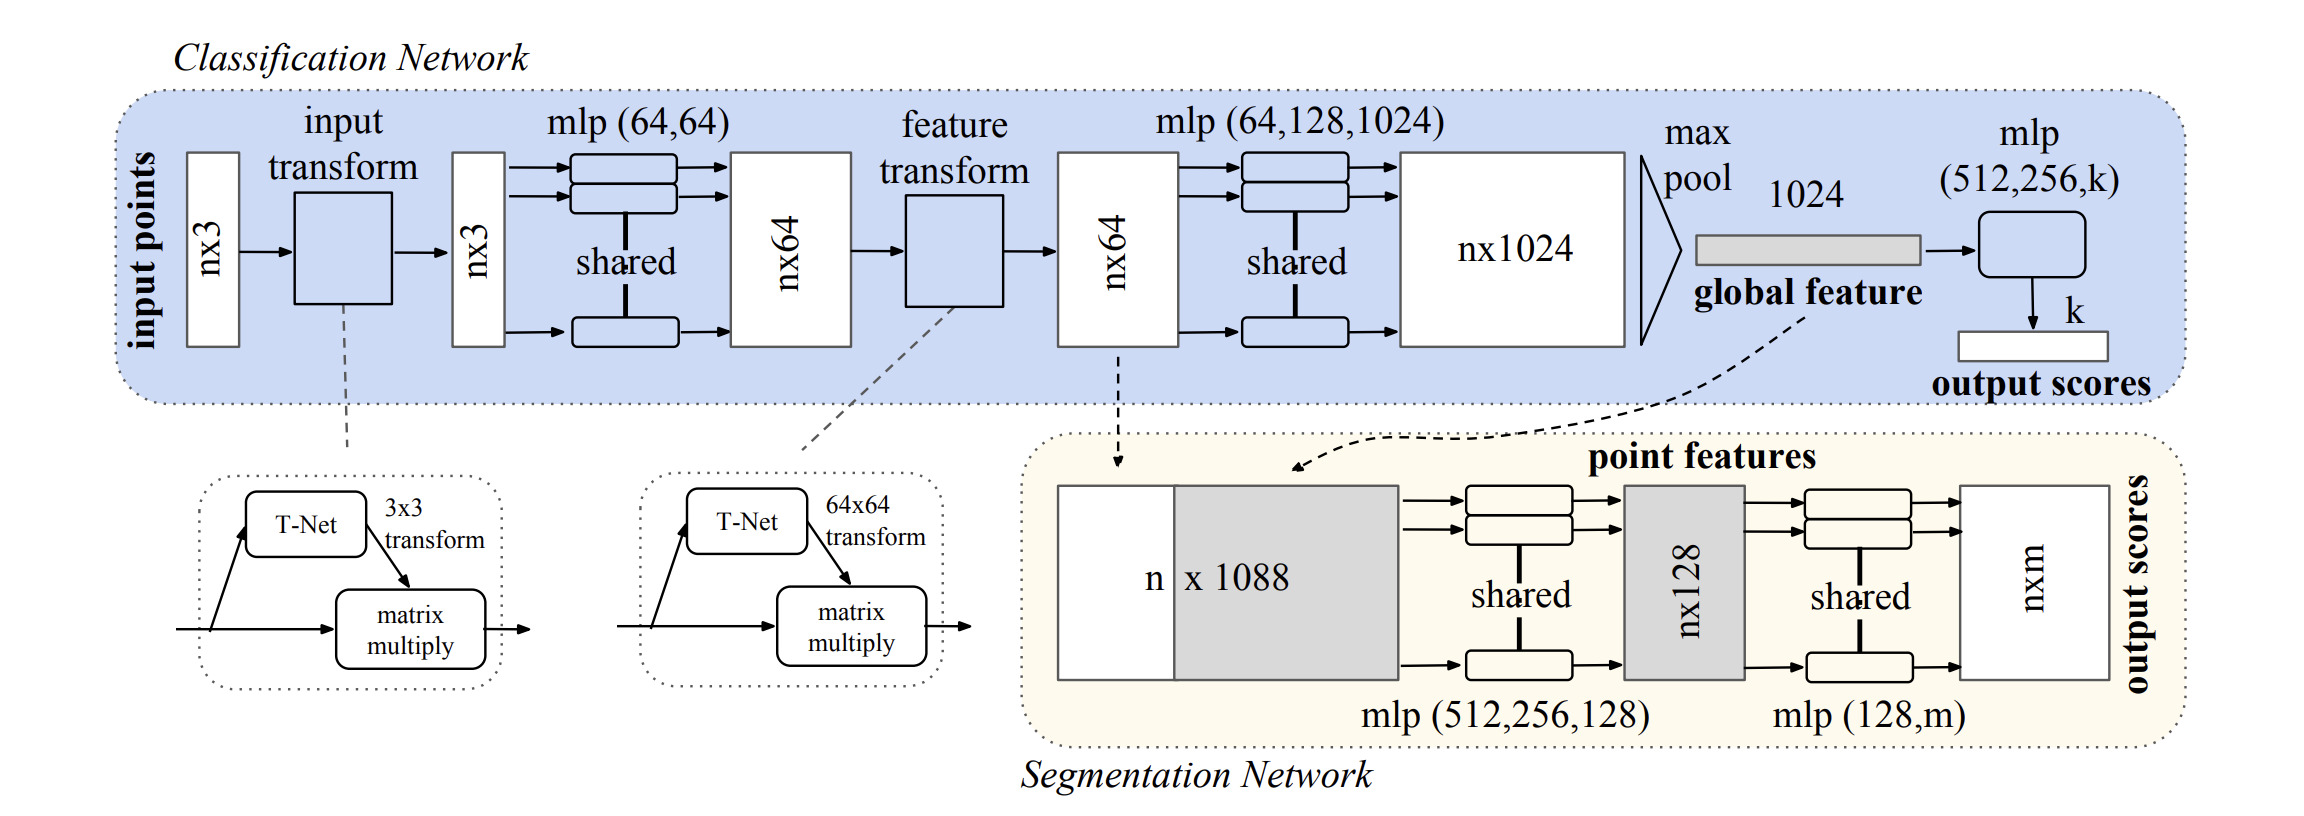
\includegraphics[width=\textwidth]{../images/pointnet_architecture.jpg}
}
\caption{\label{fig-pointnet-architecture}PointNet architecture. Figure
from (Qi, Su, et al. 2017)}
\end{figure}

\citet{qiPointNetPlusPlus2017} introduces PointNet++, aimed to address the main drawbacks of the original PointNet model, namely the use of only two scales for context encoding – per-point and global, which limits the ability of the model to respond to local structures and fine patterns and thus work in complex scenes.
To address this, PointNet++ uses a hierarchical architecture that applies PointNet recursively on nested subsets of the original point set, allowing to learn features on multiple of increasing scales.
To achieve that, network uses stacked set abstraction layers, that first sample a subset of the point cloud using farthest point sampling – an algorithm aimed to create representative subsets even for point clouds with uneven point density that selects the next point by maximizing its distance to already selected set – then constructs a neighborhood around each selected point using either fixed distance or fixed number of neighbors, and finally applies PointNet to each neighborhood to reduce into a feature vector for the sampled point.
Then, similar to the original PointNet, the subset can be further reduced to a final global feature vector used for point clouds classification, or passed to an upscaling branch with skipped connections and k-nearest neighbors interpolation to extrapolate features to the original point cloud coordinates.
The architecture is visualized in Figure~\ref{fig-pointnet2-architecture}.

\begin{figure}
\centering{
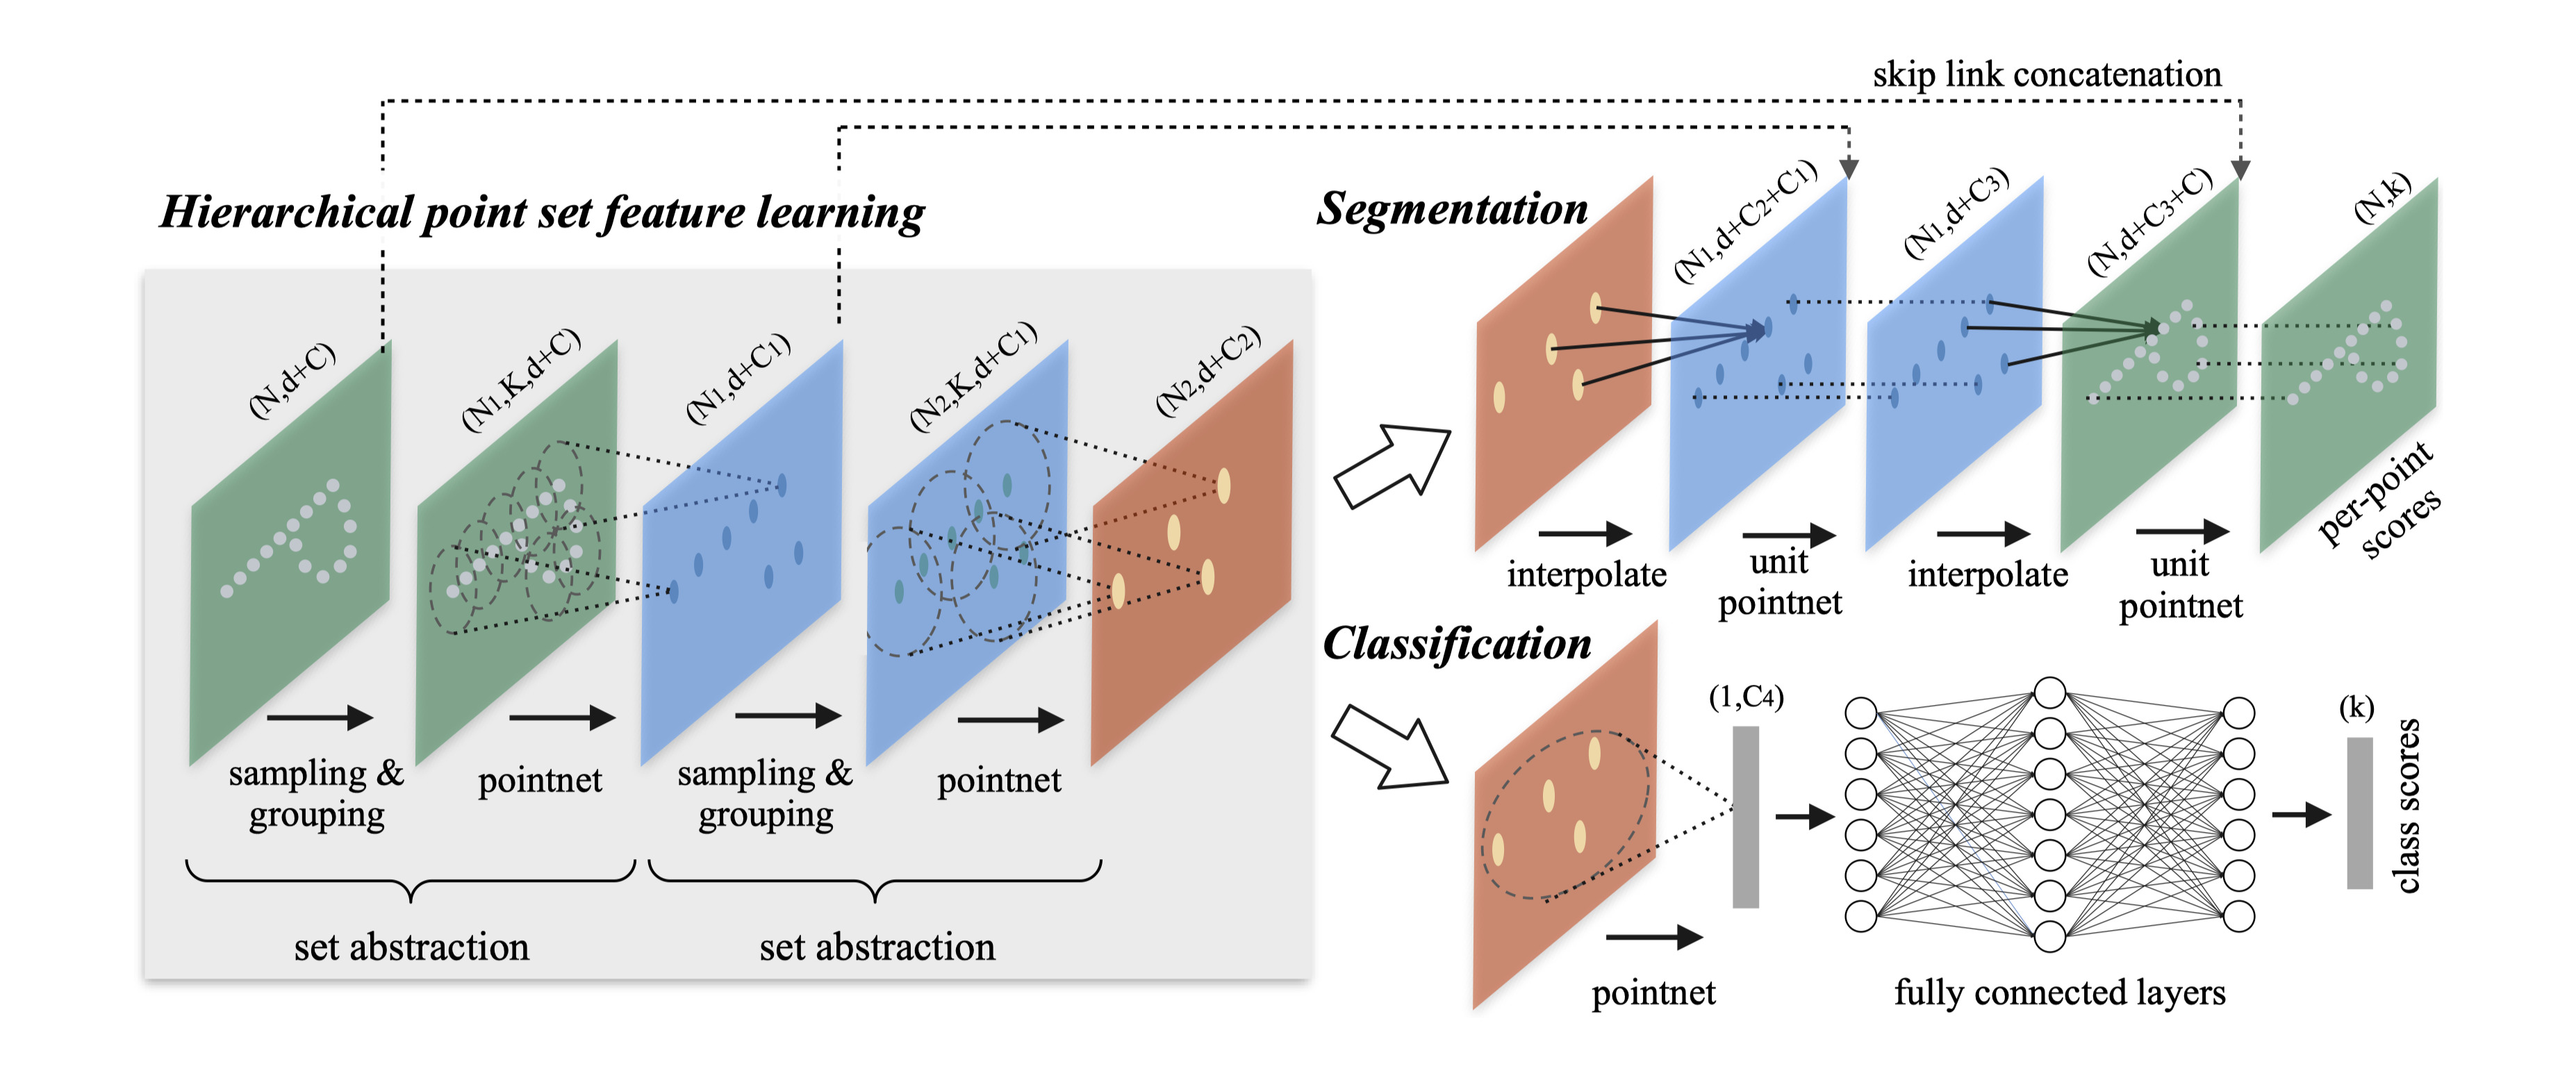
\includegraphics[width=\textwidth]{../images/pointnet2_architecture.jpg}
}
\caption{\label{fig-pointnet2-architecture}PointNet++ architecture.
Figure from (Qi, Yi, et al. 2017)}
\end{figure}

\section{Area-based approach}\label{sec-area-based-approach}

The most common way to use LiDAR for mapping forest attributes is the area-based approach \cite{whiteABAGuide2013}.
Figure~\ref{fig-aba-schema} shows its schematic representation.
It consists of a LiDAR survey covering the whole area of interest and a manual forest inventory providing ground truth data for fitting statistical models and validating the results.
The inventory usually consists of many circular ground plots with every tree within counted and attributes of interest either directly measured or calculated and averaged.
The point cloud is clipped by the extents of the ground plots, and for each plot it is reduced to a collection of manually selected metrics.
The metrics usually include descriptions of the height distribution of the points, but often reflection intensities and other sensor-provided information is used as well, such as the return number, the number of returns, etc. (a brief discussion on the use of intensity-based features can be found in Section~\ref{sec-intensity-based-features}).
In general, any summary statistic that can be derived from a collection of points can be used, including features mentioned in Section~\ref{sec-ml-dl}.
These metrics are then used as input features for fitting regression and classification models to predict the forest attributes measured on the corresponding plots.
The same metrics are calculated for the entire area of interest, using a grid with a cell size similar in area to the area of a single ground plot.
The models are then applied to the grid, generating an extrapolation of the required attributes.

\begin{figure}
\centering{
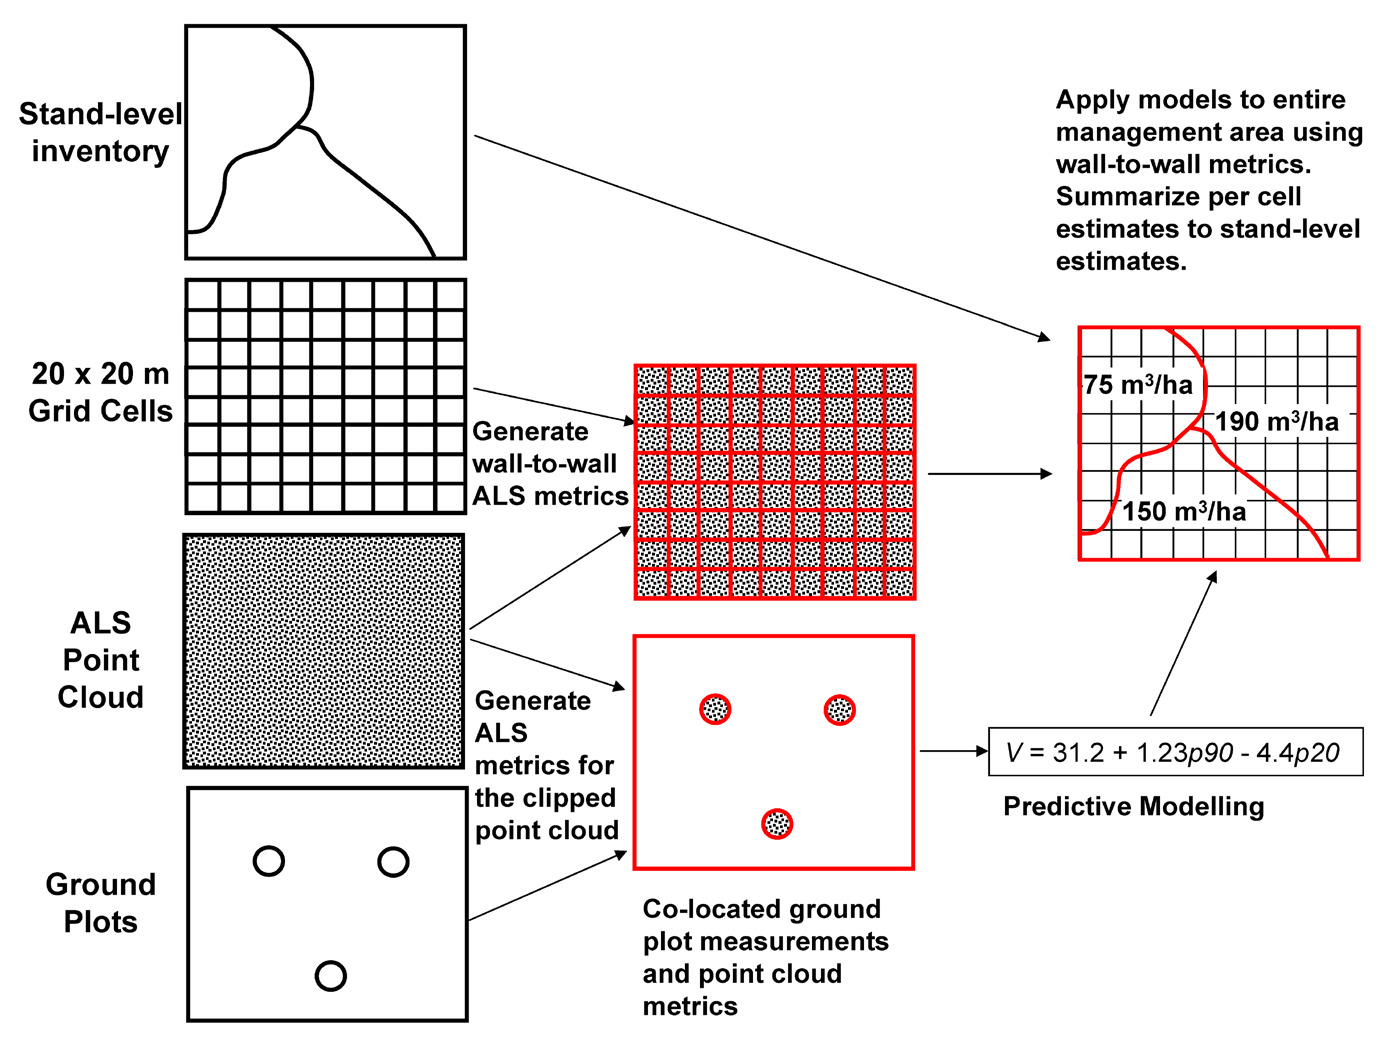
\includegraphics[width=\textwidth]{../images/aba_schematic.jpg}
}
\caption{\label{fig-aba-schema}Area-based approach schematic. Figure
from (White et al. 2013)}
\end{figure}

Area-based approach is extensively used both in research and in industry because it provides many advantages.
It is relatively easy to implement.
In fact, basic familiarity with the R programming language is enough to create your own area-based approach pipelines since a full, scalable implementation exists in the `lidR` package \cite{rousselLidRPackage2020}.
It is also straightforward to extend with other data sources such as satellite or aerial images, and it works even with sparse data: for successful plot and stand level modeling point densities as low as 0.5 points per square meter have been reported to be enough \cite{treitzLiDARSamplingDensity2012, jakubowskiTradeoffsLidarPulse2013}.
Still, it requires a lot of field inventory data to work, since every ground plot becomes a single example for the models.
The models that can be used are also relatively simple, because of how expensive the data collection is.
Data-hungry approaches like neural networks usually don't have enough data to train.
The results are also very coarse – predicted on a grid with the size defined by the area of a plot (a common plot shape is a circle with 9-meter radius, which is approximately equivalent to a square grid cell with 16-meter side).
This is why they are usually further aggregated to stand level.

\subsection{Examples of studies using ABA}

\citet{bouvierGeneralizingPredictiveModels2015} suggest a set of 4 metrics they use to fit models for predicting timber volume, above ground biomass, and basal-area on stand level, instead of most commonly used metrics based on the distribution of height.
Their metrics are aimed to capture different aspects of the canopy geometry.
The authors argue that usage of a very limited set of carefully engineered diverse metrics results in improvement of model generalization ability without loss of accuracy.

\citet{zhangImprovedAreabasedApproach2023} use a modification of the area-based approach to predict plot-level diameter at breast height (dbh) by utilizing known allometric dependencies between tree height and dbh to limit size of the hypothesis set for fitting regression models.
They use airborne LiDAR measurements with an average density of 9.6 points per square meter and report a relative error of 11\%.

\citet{vermeerLidarbasedNorwegianTree2023} use a U-Net \citep{ronnebergerUNetConvolutionalNetworks2015} image semantic segmentation model on LiDAR-derived 1-meter resolution digital terrain models and canopy height maps to predict the distribution of three main tree species in a Norwegian forest.
They achieve a macro $F_1$ of 0.70 when including the background class, and 0.63 when including only the target species classes, as evaluated on independent field inventory plots.

\citet{kcEstimationAboveGroundForest2024} is a classic example of an area-based approach study utilizing airborne LiDAR survey to predict forest above ground biomass.
They use a set of 32 metrics derived from height distribution of points, an automatic feature selection procedure, and two regression models: linear regression and Random Forest to compare the results.
They report coefficients of determination of 0.85 and average errors around 83 tons per hectare.

\section{Individual tree-based approach}\label{sec-individual-tree-approach}

\citet{liNewMethodSegmenting2012} developed a well performing algorithmic method for segmentation of individual tree crowns in LiDAR point clouds for coniferous forests that relies on the pointy shape characteristic of many coniferous species and segments the trees from top to bottom.

\citet{lucasIdentificationLinearVegetation2019} use the set of eigenvalue-based features calculated for each point in a fixed-radius neighborhood, with other geometrical features including maximum local height difference and height standard deviation, local radius and local point density, to identify linear vegetation elements in segmented point clouds.
They also use two point-based features that don't rely on a neighborhood: the number of returns and the normalized return number, proposed in \citet{guoRelevanceAirborneLidar2011}, and use Random Forest classifier to separate the points that belong to vegetation after first removing the planar features corresponding to grass, soil, and water surfaces.
The approach is somewhere in the middle between the area-based and individual tree-based, but still is a useful example of application of classic machine learning to segment out vegetation from larger point clouds.

\subsection{Image-only}

Many approaches rely only on images, mostly high-resolution RGB and multispectral ones, but lately also hyperspectral.
The main advantage of such approaches is a well-established and well-known toolbox in terms of both algorithmic processing and deep learning, as many of the most important deep learning milestones were achieved in the field of computer vision.
They also can rely on consistent resolution, capture of fine details and textures, and continuous representation of sensed environments.
The main disadvantages were mentioned in the introduction: passive sensors rely on the sun as the source, and thus greatly depend on lighting such as cloud and terrain shadows, time of day, season.
They also offer no information on vertical structure.
Still, they are very popular and achieve outstanding results in many environments.

\citet{weinsteinDeepForestPythonPackage2020} introduces a Python package for training and inference of ecological object detection neural networks in airborne imagery.
It uses a convolutional object detection network described in \citet{weinsteinIndividualTreeCrownDetection2019} to predict bounding boxes for individual trees.
The data the model is trained on is not as dense as the forests that are the target of this thesis.
Moreover, the model requires fine-tuning to be applicable to new data, which greatly limits its applicability, since developing bounding box annotations for individual trees within dense forests is an extremely tedious and labor-intensive task.

\citet{lassalleDeepLearningbasedIndividual2022} use high-resolution satellite imagery to delineate individual tree crowns in mangrove forests by using DeepLabv3+-based Multi-Task Encoder-Decoder network (MT-EDv3) originally proposed by \citet{larosaMultitaskFullyConvolutional2021} to predict for each pixel the distance to the tree crown border.
This distance map is then enhanced by applying the Laplacian over Gaussian filter, and finally the watershed segmentation algorithm is applied to delineate individual crowns.
The approach seems to rely on there being semi-clear separation between the tree crowns, which is rarely the case when the forests are dense and mixed.

The same network was also successfully used to map tree species in tropical urban environment in Rio de Janeiro, Brazil in \citet{martinsDeepLearningbasedTree2021}.
They develop a post-processing approach to combine the semantic segmentation map and the distance map to classify tree species with an average $F_1$-score of 79.3% and resulting in a realistic tree species map.

\citet{oscoConvolutionalNeuralNetwork2020} use a convolutional neural network on UAV multispectral images to count citrus trees in an orchard by predicting a confidence map that shows the likelihood of each pixel containing a tree.
They report $F_1$-scores of up to 0.95, which is impressive even for managed stands.

\citet{venturaIndividualTreeDetection2024} describe a network they call HR-SFAnet, consisting of a VGG-16 \citep{simonyanVeryDeepConvolutional2014} backbone feature extractor, a confidence head, and a parallel attention head, for detecting individual trees in urban environments using high-resolution multispectral images.
The network is a deeper modification of the SFANet proposed in \citet{zhuDualPathMultiScale2019} for counting the number of people in photos.
They report $F_1$-scores of 0.75, with average positioning error of 2.2 meters.

\subsection{Terrestrial LiDAR}

Terrestrial LiDAR surveys usually provide very dense and detailed point clouds.
Most importantly for the task of localizing individual trees, terrestrial measurements always capture the trunks of the trees clearly.
Tree trunks are very useful for tree detection and segmentation, and there are many algorithms that use bottom-to-top approaches that trace the trunks into the canopies.

\citet{burtExtractingIndividualTrees2018} introduce `treeseg`, a software package written in C++ for extracting individual trees from LiDAR point clouds.
Even though it is designed and presented as platform-agnostic methods made to operate on both terrestrial and UAV LiDAR point clouds, it relies on trunk detection, which is common for many methods based on terrestrial LiDAR and often is not applicable to UAV LiDAR data.

\citet{lopezserranoArtificialIntelligencebasedSoftware2022} introduce another software package called `AID-FOREST` for fully automatic processing of terrestrial LiDAR point clouds based on trunk detection.
The software takes in a raw point cloud, performs all required preprocessing steps, and runs an object detection neural network on a series of horizontal slices to find cross-sections of trunks, and then processes the detection results from each level to track individual trees.

\citet{allenTreeSpeciesClassification2022} describe an approach for classifying terrestrial LiDAR point clouds of individual trees extracted by `treeseg` using multi-view representation based on \citet{goyalRevisitingPointCloud2021} and a convolutional ResNet network \citep{heDeepResidualLearning2016}.
They report high classification accuracies both overall and per-species on a dataset of almost 2500 individual trees.

\citet{wilkesTLS2treesScalableTree2023} introduce `TLS2trees`, another automated framework for segmentation of individual trees in terrestrial LiDAR point clouds, consisting of a set of Python command line tools.
The framework consists of three steps: preprocessing, semantic segmentation, and instance segmentation into a set of individual trees.
After that, a set of attributes are computed for each tree.
The software is designed to be horizontally scalable (meaning it's easy to speed up calculations by using more machines doing them in parallel, as opposed to vertically, meaning by increasing the computational resources available to a single machine) to address huge datasets produced during terrestrial laser scanning surveys.

All these software packages are impressive, but non-applicable to the data described in this work.

\citet{vianaTimberVolumeEstimation2022} use a small dataset to compare tree-level inventory metrics extracted from a terrestrial LiDAR survey and from a manual inventory.
They report very good results, showing that terrestrial LiDAR can serve as a replacement for manual inventories in diverse secondary forests (secondary forests are forests that regenerate naturally after significant disturbances like logging, storms, or fires).

\citet{nurunnabiDevelopmentPreciseTree2024} offer a compelling example of how detailed terrestrial LiDAR point clouds can be used to provide very detailed analyses on tree level.
The authors report high accuracies on the task of segmenting the point clouds into wood and leaf points by utilizing geometric features mentioned earlier to locate linear and non-linear areas.
They then apply an octree-based segmentation algorithm to develop a precise 3D structure of a tree.

\subsection{UAV LiDAR}

A common approach to utilize LiDAR point cloud data for tree detection is by calculating canopy height maps – images where each pixel represents the height of vegetation – and applying the same techniques as for image-only approaches.

A substantial number of different tree detection algorithms are variations of the local maxima filter, differing in what the filter is applied to, how many times, with what windows, and how the results are combined or preprocessed.
For example, \citet{doussExtractionIndividualTrees2022} offers an exploration of how different window size functions for the local maxima filtering applied to LiDAR-derived canopy height maps affect the quality of individual tree detection.
They show that for a moderately dense forest in France, it is possible to find the parameters for the local maxima filter window that produce satisfactory results.
It is, however, clear that it requires great deal of manual adjustment, and visual inspection of the results of detection makes it clear that they are only locally consistent.
Any change in the canopy structure patterns noticeably affects the quality of the detection even for sophisticated window functions.

\citet{lisiewiczCorrectingResultsCHMBased2022} propose a way to improve the results of canopy height map-based individual tree detection algorithms.
Their approach consists of three steps.
The first step is the classification of segments into correct, under-segmented, or over-segmented using a Random Forest classifier, the second step is the refinement of under-segmentation errors by re-segmenting them with adjusted parameters, and the last step is the refinement of over-segmentation errors by merging with the correct segments using an algorithmic approach based on a collection of intensity-derived features.
The authors suggest that this approach is universal in terms of forest composition and complexity, unlike many other ad-hoc correction methods based on the study area and thus non-generalizable.

\citet{wangAutomaticDetectionIndividual2023} propose a two-stage network they call Tree Region-Based Convolutional Neural Network (RCNN) to detect trees in UAV LiDAR point clouds.
The first step is generation of dense anchors across the point cloud that are then processed by the RCNN to generate proposals for individual tree locations.
The second step involves multi-position feature extraction to refine the proposals.
The approach is evaluated on the NewFor benchmark \citep{eysnAlpineITDBenchmark2015} and outperforms all benchmark methods that come with it.

\citet{fuIndividualTreeSegmentationUAV2024} propose a method for segmenting individual trees in UAV LiDAR point clouds based on a multiscale adaptive local maximum filter applied to the smoothed canopy height map to detect tree tops, a region-growing method for crown delineation that are then refined a voxel-based clustering algorithm.
The method is developed and tested on 21 synthetic plots and one actual survey and the authors report good accuracy for estimation of both tree locations and heights.
Worth noting that both the synthetic and real forest have relatively well defined an unambiguous canopy structure.

\subsection{Fusion of data}

\citet{lianBiomassCalculationsIndividual2022} describe an approach for calculating individual tree biomass by combining UAV multispectral, UAV LiDAR and terrestrial LiDAR data.
Terrestrial and UAV LiDAR a merged to get a more representative point cloud, showing the trees equally well both from above and from the ground.
The multispectral image is used to generate a species classification map, which is then used to segment the point cloud.
The segmented cloud is then used to estimate diameter at breast height and height and calculate above ground biomass.

\citet{liFusionApproachesIndividual2023} explore the contributions of multispectral images, very high resolution panchromatic images, and LiDAR data during fusion on feature and decision level for tree species classification using Support Vector Machine and Random Forest classifiers on manually delineated tree crowns from an urban environment.
They report that fusion consistently improves the results over using each of the data sources on its own.
They also report that fusion on decision level resulted in the highest overall accuracy metrics.

\citet{balestraLiDARDataFusion2024} offers a review of 151 publications concerning fusion of LiDAR data with other remote sensing data.
The authors report that in most cases fusion improves the results.
Most relevant to this thesis, they report that for individual tree segmentation the results of fusion-based approaches compared to LiDAR-only ones are consistently better.
\citet{laExtractionIndividualTree2015} show an increase from 63\% to 92\% for low-density forests, and from 62\% to 70\% for high-density forests, \citet{aubry-kientzMultisensorDataFusion2021} show and improvement by 5\%, and \citet{zhenImpactTreeOrientedGrowth2014} and \citet{arenas-corralizaAutomaticMappingTree2020} improved their results by 2-4\%.

\citet{ferreiraImprovingUrbanTree2024} use a U-Net semantic segmentation model for fusion of VNIR images and UAV LiDAR-derived feature maps including surface normals of the canopies, reflection intensities, canopy heights, and leaf-area index for mapping tree species in urban tropical areas.
Their results show that adding LiDAR-based features improves $F_1$-scores across all considered species, with average $F_1$-score 84.1.
They also use the segment anything model \citep{Kirillov_2023_ICCV} to automatically segment tree crowns with outstanding 98\% boundary $F_1$-score.

\citet{wuFineClassificationUrban2024} use a combination of high-resolution RGB images and LiDAR to classify urban tree species by extracting seven different feature types and using a Random Forest for pixel-level classification.
They report on seven experiments using different combinations of extracted features.
The results show an improvement of 18.5\% in accuracy when using fusion of LiDAR and RGB compared to RGB-only.

\subsection{Summary}

That's how it is.
\chapter{Materials and methods}\label{cap:materials}

This chapter describes in detail used datasets, processing techniques and the methods, and comments on the reasoning behind the choices.
The code of the project on my GitHub might be a helpful addition for that.


\section{Lysva dataset}\label{sec-lysva-dataset}

The main original dataset used in the study is the Lysva field inventory dataset, named by the closest town to its location.
The dataset is released into open access with an accompanying paper that describes the data in detail and provides a basic baseline for individual tree detection \citep{dubrovinExplorationPropertiesPoint2024}.
The study area is located in Perm Krai, Russia, 86 kilometers to the east of Perm.
The forest in the region is natural, with the average age of coniferous trees over 85 years and deciduous over 60 years.
The dataset consists of a field inventory of 3600 trees across 10 rectangular ground plots 100 meters in lengths and 50 meters in width fully covered by a \gls{uav} \gls{lidar} and \gls{rgb} orthophoto surveys.
Figure~\ref{fig-lysva-roi} shows the locations of the ground plots over the full size \gls{rgb} orthophoto and a visualization of the field inventory for a single plot on top of the \gls{lidar} point cloud.
The low vegetation areas visible on the orthophoto are naturally regenerating old logging and agricultural sites.
No artificial afforestation has been done in the area.
Colored points represent trees, with different colors mapping to different species.
The point cloud is visualized as a 2D scatter plot with points colored by height (darker points are lower, brighter points are higher, and points are unsorted – some lower points end up over higher ones).
The baseline is a simple one-pass local maxima filter applied directly on the point cloud with a fixed window size.

\begin{figure}
\centering{
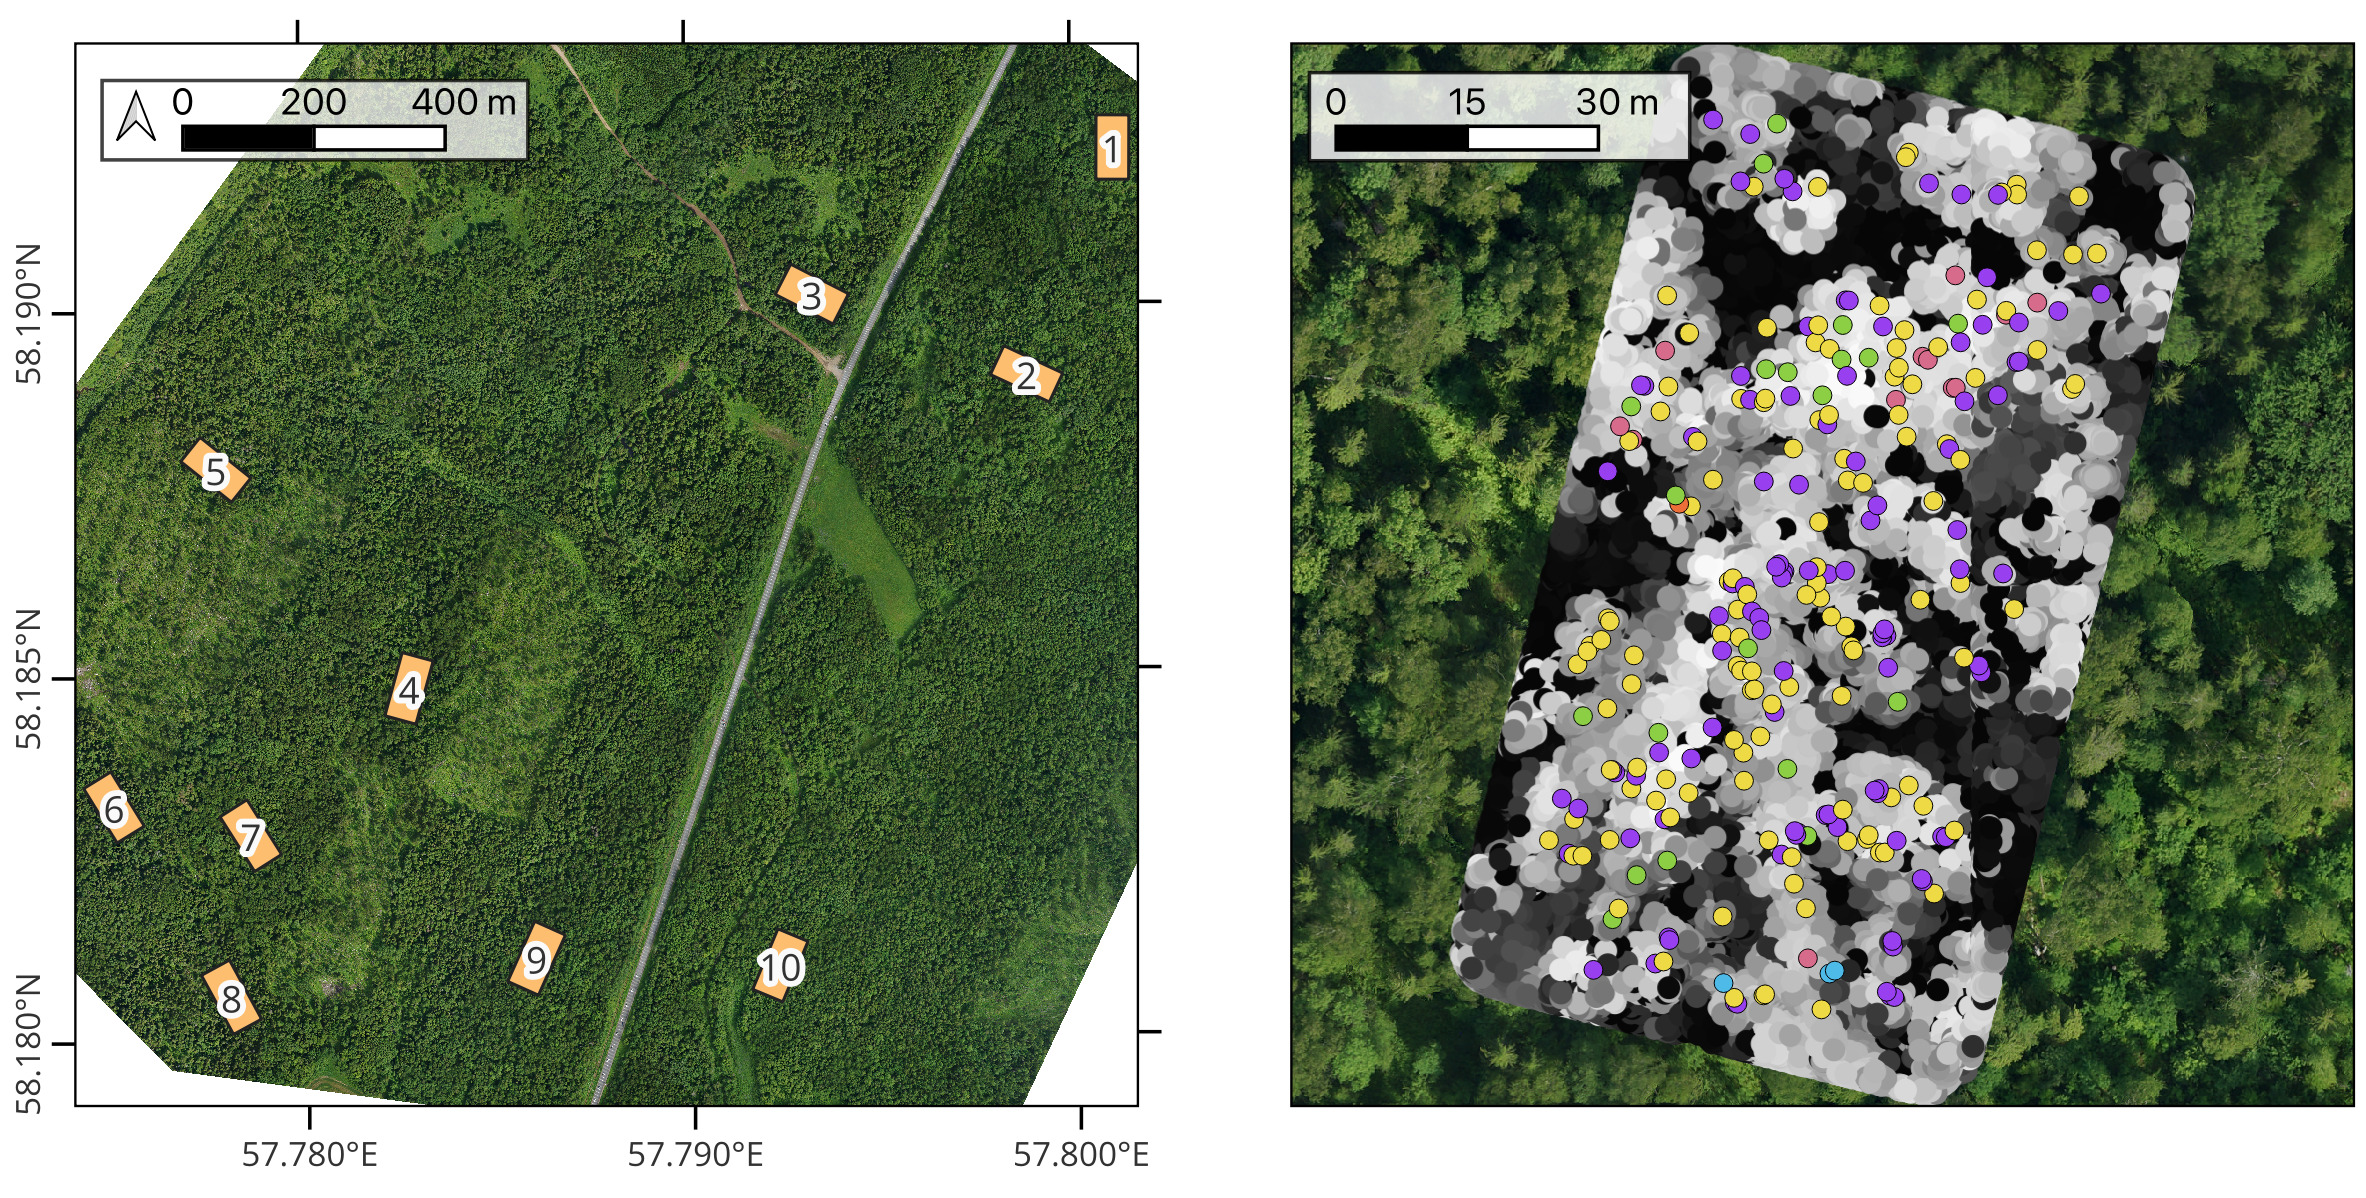
\includegraphics[width=\textwidth]{../images/lysva_roi.jpg}
}
\caption[The study region for the Lysva field inventory.]{\label{fig-lysva-roi}The study region for the Lysva field
inventory dataset. \textbf{Left}: The locations of field survey plot
boundaries on a full-size RGB orthophoto. Each plot is a 50 by 100 meter
rectangle, with every tree with dbh of 6.1 cm or higher measured and recorded. Buffered
cutouts of the orthophoto come with the dataset, along with LiDAR point
clouds. \textbf{Right}: A close up of plot number 4. Each colored point
represents a single tree of a different species, on top of a point cloud
colored by the value of the height of each point (lower points are dark,
higher points are bright) and the same orthophoto.
Note that the points of the point cloud are unsorted, and some lower points overlap higher points.
Figure reused from \citet{dubrovinOpenDatasetIndividual2024}.}
\end{figure}


The field inventory is a tabular dataset where every row represents a single tree.
According to the state-mandated requirements that were in place during the collection of the data, all trees with \gls{dbh} starting from 6.1 centimeters were included.
Table~\ref{tbl-inventory-example} shows a random sample of entries from the field inventory table.
Every tree is represented by a point in \gls{utm} 40N coordinate reference system (\gls{epsg}:32640).
The coordinates of the trees were determined using the South NTS-360R total station with a reflector prism using the closed traverse method.
The total station measurements used two points basis determined using a dual-frequency South G1 Plus IMU \gls{gnss} receiver in \gls{rtk} mode.
The basis points were selected to have reliable satellite signal.
The average error of coordinate measurements is 10 centimeters, with a maximum of 30 centimeters.
Every tree has a species label and \acrfull{dbh}, measured with calipers at 1.3 m from the ground at two perpendicular directions and averaged.
Figure~\ref{fig-lysva-species-distribution} shows the distribution of species in the data: the dominant species is spruce, but overall the trees are evenly split between deciduous and coniferous, 1793 and 1807 respectively, with seven species in total: spruce, birch, fir, aspen, tilia, alder, and willow.
Approximately 20\% of the trees have height data measured during the inventory, and 10\% have ages measured on core samples, shown in the table in meters and years respectively.


\begin{longtable}[]{@{}lllllllllll@{}}

\caption[Example of data in the field inventory table.]{\label{tbl-inventory-example}Example of data in the field
inventory table. Each row is a recorded tree and is represented by a point in UTM 40N coordinate reference system (EPSG:32640). Coordinates are not shown.}

\tabularnewline

\toprule\noalign{}
Plot & Tree ID & Species & $d_1$ & $d_2$ & dbh & Age & Height & Angle &
Comment \\
\midrule\noalign{}
\endhead
\bottomrule\noalign{}
\endlastfoot
7.0 & 111.0 & Birch & 23.0 & 23.0 & 23.00 & – & – & 0.0 & – \\
5.0 & 136.0 & Fir & 23.5 & 23.0 & 23.25 & 90.0 & 17.5 & 0.0 & Rotten \\
3.0 & 119.0 & Aspen & 36.1 & 42.1 & 39.10 & 89.0 & 25.5 & 0.0 & – \\
9.0 & 345.0 & Spruce & 19.7 & 22.0 & 20.85 & – & 15.9 & 0.0 & – \\
6.0 & 267.0 & Spruce & 12.9 & 12.9 & 12.90 & – & – & 0.0 & – \\

\end{longtable}

\begin{figure}
\centering{
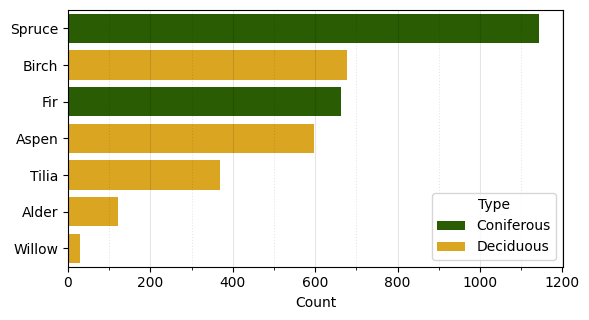
\includegraphics[width=\textwidth]{../images/03a_lysva_dataset-fig-lysva-species-distribution-output-1.png}
}
\caption[Distribution of species in the Lysva field inventory dataset]{\label{fig-lysva-species-distribution}Distribution of species
in the Lysva field inventory dataset. The dominant species is spruce,
but overall the split between coniferous and decidious species is even:
there are 1807 coniferous and 1793 deciduous trees.
Figure reused from \citet{dubrovinOpenDatasetIndividual2024}.}
\end{figure}

The \gls{lidar} sensor used for the survey is AGM-MS3 produced by AGM Systems.
It has 640 kHz acquisition rate, 300-meter range, and spatial accuracy of 3–5 centimeters.
The raw point clouds were processed with the combination of the AGM ScanWorks software from the sensor vendor and the TerraScan software.
The point clouds were preprocessed by removing duplicate points and high and low noise points.
The duplicate removal was run with a threshold distance between points of 1 mm.
Noise was removed by visually inspecting the point cloud and manually selecting height thresholds to cut off points that are lower than the ground or higher than the canopies.
Ground point classification was performed and ground points were used to normalize height by subtracting the ground level from the Z coordinate of every point.
Height normalization allows treating the Z coordinate as height above ground rather than the absolute elevation, which simplifies many subsequent steps.
The camera used to collect raw digital images for creating the orthophoto is Sony A6000.
Agisoft Metashape software was used to generate the orthophoto mosaic.
A canopy-height map was created from the \gls{lidar} point cloud and used as a reference for adjusting the planar coordinates of the orthophoto to align them.
The resolution of the orthophoto is 7 centimeters per pixel.
Figure~\ref{fig-example-3d-point-cloud} is a 3D visualization of the point cloud over plot number 10.
It shows the unmodified point cloud on the left, with points colored by height above ground, and a point cloud enriched with color information by sampling the orthophoto at the planar coordinates of the points.
Figure~\ref{fig-example-ortho} shows the orthophoto for the same plot.
The carrier \gls{uav} used for the \gls{lidar} survey is DJI Matrice 600 Pro hexacopter.
The speed during the survey was 10 meters per second.
The \gls{uav} was configured to follow the terrain at 150 meter height using the \gls{srtm} elevation map as a reference \citep{farrShuttleRadarTopography2000}.
The carrier \gls{uav} used for the orthophoto survey is the fixed-wing Geoscan 201 Geodesy.
The speed during the survey was 16.6 meters per second.
Figure~\ref{fig-uavs} shows the \glspl{uav} used for the remote sensing data collections.
Table~\ref{tbl-lysva-equipment} summarizes the sensor and platform characteristics, as well as some of the acquisition parameters.

\begin{figure}
\begin{minipage}{0.50\linewidth}
\centering{
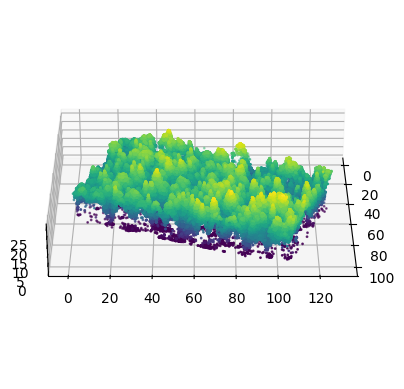
\includegraphics[width=\textwidth]{../images/03a_lysva_dataset-fig-example-3d-point-cloud-output-1.png}
}
\subcaption{\label{fig-example-3d-point-cloud-1}Points colored by
height.}
\end{minipage}
\begin{minipage}{0.50\linewidth}
\centering{
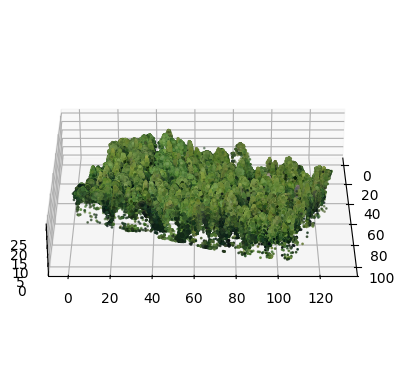
\includegraphics[width=\textwidth]{../images/03a_lysva_dataset-fig-example-3d-point-cloud-output-2.png}
}
\subcaption{\label{fig-example-3d-point-cloud-2}Points assigned color by
sampling the orthophoto.}
\end{minipage}
\caption{\label{fig-example-3d-point-cloud}A 3D visualization of the UAV
LiDAR point cloud of plot 10.}
\end{figure}

\begin{figure}
\centering{
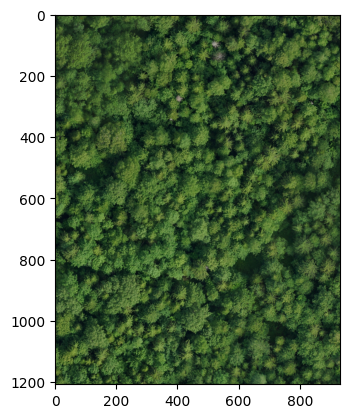
\includegraphics[width=\textwidth]{../images/03a_lysva_dataset-fig-example-ortho-output-1.png}
}
\caption{\label{fig-example-ortho}A visualization of the orthophoto of
plot 10.}
\end{figure}

\begin{figure}
\centering
\begin{subfigure}[b]{0.45\textwidth}
    \centering
    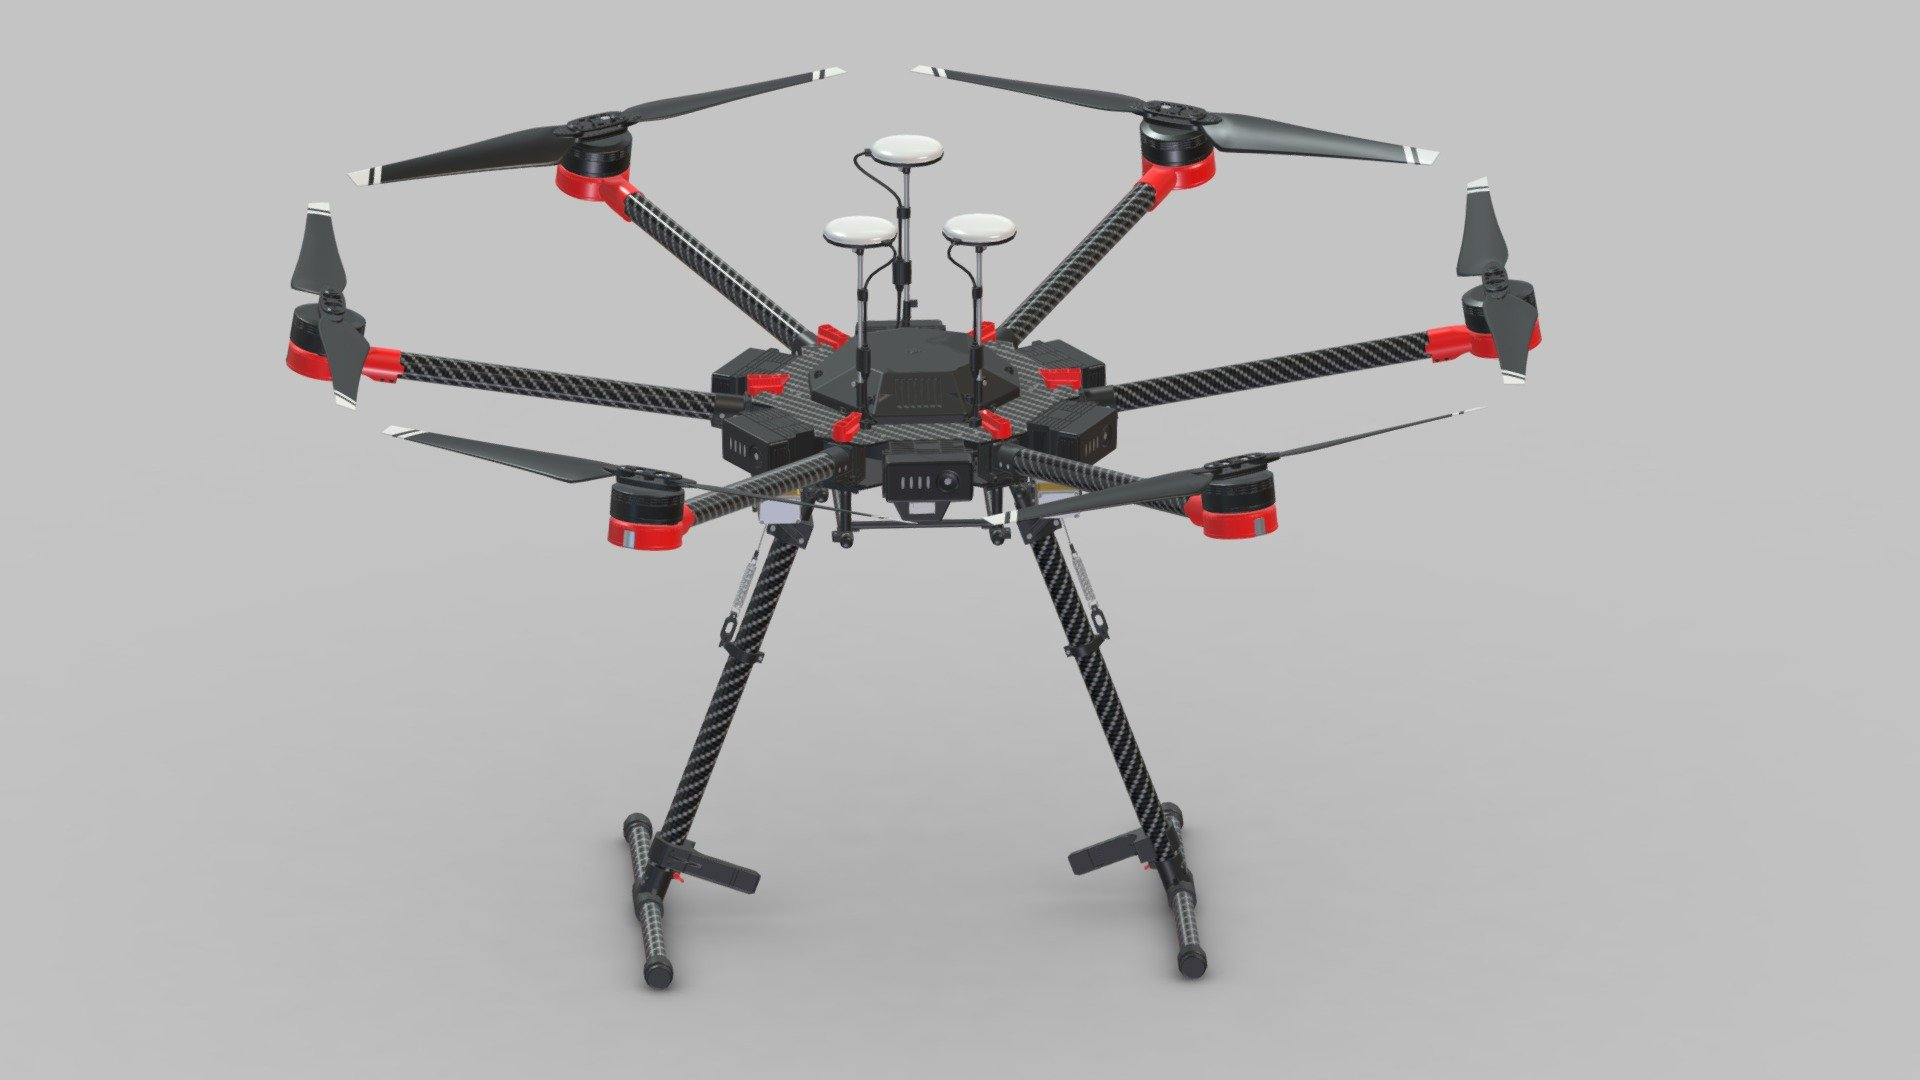
\includegraphics[width=\textwidth]{../images/dji-matrice-600-pro.jpeg}
\end{subfigure}
\hfill
\begin{subfigure}[b]{0.45\textwidth}
    \centering
    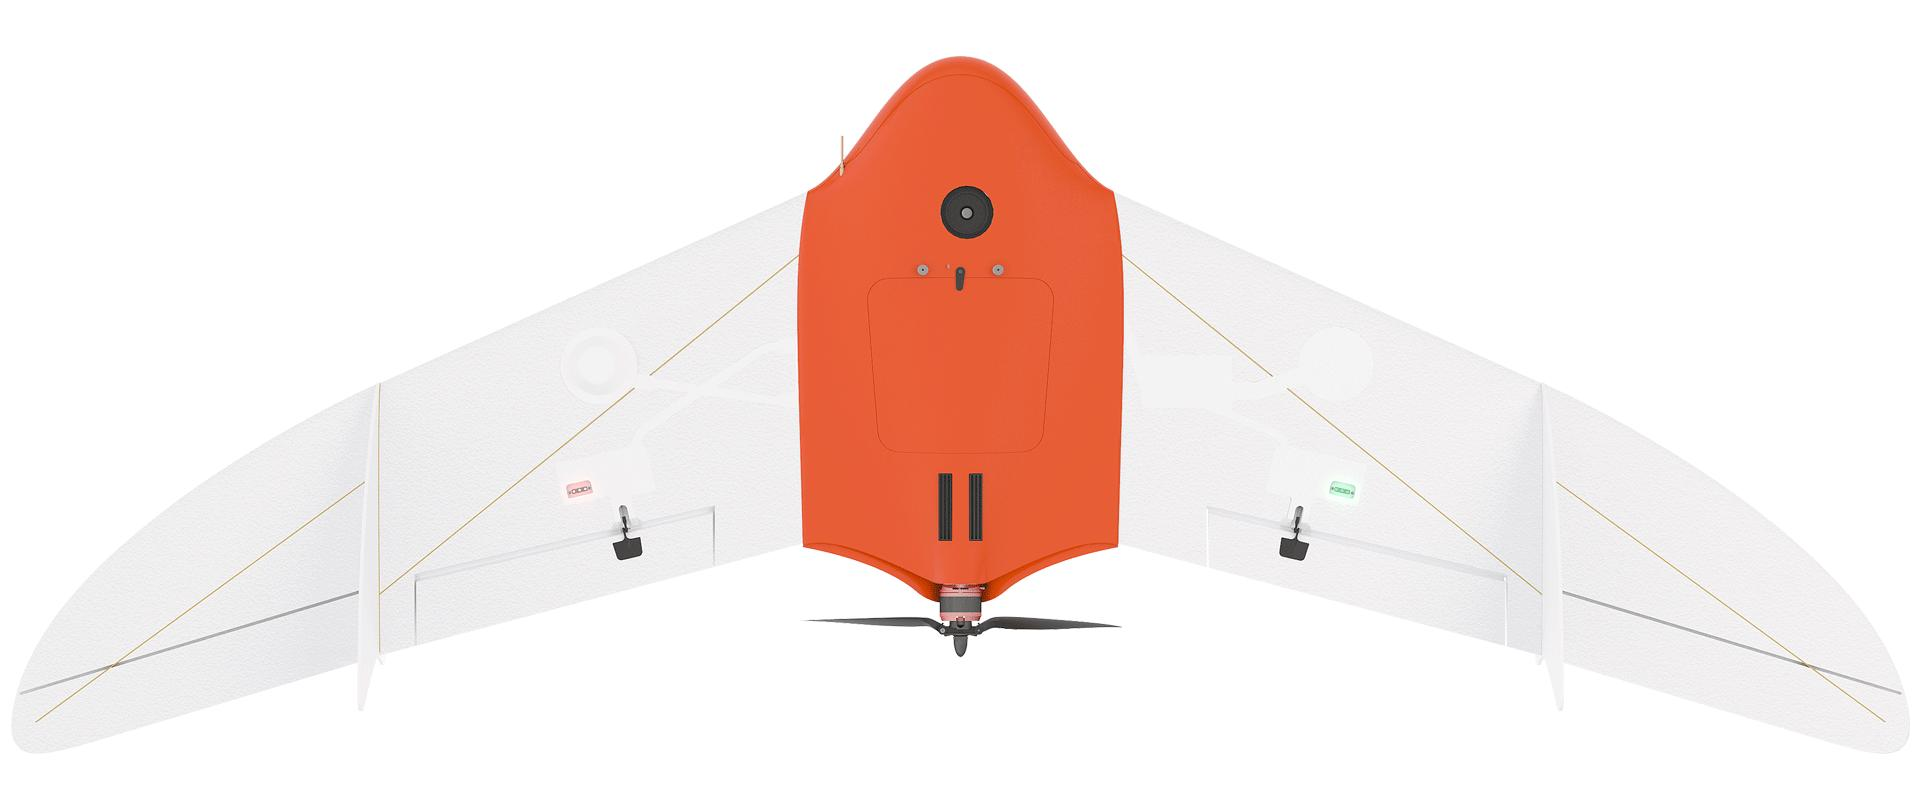
\includegraphics[width=\textwidth]{../images/geoscan_201_geodesy.jpg}
\end{subfigure}
\caption[UAVs used for data collection.]{
    UAVs used for data collection (photos from vendor websites).
    \textbf{Left}: DJI Matrice 600 Pro that was used for the LiDAR survey.
    \textbf{Right}: Geoscan 201 Geodesy that was used for the orthophoto survey.
}
\label{fig-uavs}
\end{figure}

\begin{table}
    \centering
    \caption{Summary of the equipment used for remote sensing data collection in for the Lysva dataset.}
    \label{tbl-lysva-equipment}
    \begin{tabular}{rll}
        & \textbf{LiDAR survey} & \textbf{Orthophoto survey} \\
        \toprule
        \textbf{Sensor} & AGM-MS3 & Sony A6000 \\
        \textbf{Resolution} & 37 points/m² & 7 cm/px \\
        \textbf{Carrier UAV} & DJI Matrice 600 Pro & Geoscan 201 Geodesy \\
        \textbf{Carrier UAV type} & Rotary-wing (hexacopter) & Fixed-wing \\
        \textbf{Acquisition height} & 150 m & 150 m \\
        \textbf{Acquisition speed} & 10 m/s & 16.6 m/s \\
        \bottomrule
    \end{tabular}
\end{table}

Table~\ref{tbl-lysva-plot-stats} shows some descriptive statistics for each plot in the field inventory: the number of trees in the plot, average \gls{lidar} point density in points per square meter, and dominant species type.
The overall average point density is 37 points per square meter.
Exactly half of the plots are predominantly coniferous and half are predominantly deciduous.
Figure~\ref{fig-lysva-canopy-structure} shows two point clouds clipped by plot bounds in 3D, highlighting the differences in canopy structure complexity between predominantly deciduous and coniferous plots.
The figure highlights that the forest is indeed dense and mixed, with non-uniform, complex canopy structure.

\begin{table}
    \centering
    \caption{\label{tbl-lysva-plot-stats}Statistics for the plots in the
Lysva dataset.}
    \begin{tabular}{llll}
    \toprule
Plot & Tree count & Point density & Dominant type \\
    \midrule
1.0 & 420 & 31.7 & Deciduous \\
2.0 & 365 & 47.9 & Deciduous \\
3.0 & 332 & 40.3 & Deciduous \\
4.0 & 261 & 33.5 & Coniferous \\
5.0 & 208 & 14.2 & Coniferous \\
6.0 & 290 & 39.1 & Coniferous \\
7.0 & 408 & 41.9 & Deciduous \\
8.0 & 341 & 35.5 & Coniferous \\
9.0 & 459 & 42.1 & Coniferous \\
10.0 & 518 & 42.9 & Deciduous \\
    \bottomrule
    \end{tabular}
\end{table}

\begin{figure}
\centering{
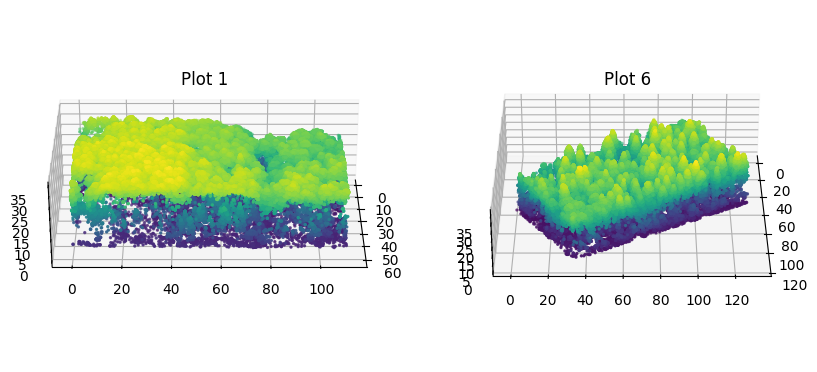
\includegraphics[width=\textwidth]{../images/03a_lysva_dataset-fig-lysva-canopy-structure-output-1.png}
}
\caption[Comparison of canopy structure in 3D point clouds.]{\label{fig-lysva-canopy-structure}3D visualizations of point
clouds from plot 1 (predominantly deciduous) and plot 6 (predominantly
coniferous). Note the difference in the canopy structure: it is
relatively easy to tell conifers apart visually, while deciduous
species do not have pronounced shapes and are hard to discriminate.
Figure reused from (Dubrovin and Fortin 2024).}
\end{figure}

\subsubsection{On using intensity-based features}\label{sec-intensity-based-features}

Even though some sources report intensity-based features as some of the most important ones \cite{shiImportantLiDARMetrics2018}, the features seem to me unreliable in the context of forestry because of the physics of light reflection.
There are simply too many factors that affect the amplitude of the reflected signal, which might be useful when imaging stable targets such as urban environments but become completely unpredictable on highly unstable targets such as trees: they move in the wind in the time span of a single survey, they grow in the time span between repeated surveys, the leaves and branches are angled in every possible way.
Moreover, the quality of the recorded intensities highly depends on the used sensor.
As an example, Figure~\ref{fig-intensity-with-example} shows the distribution of intensity values for every point in the Lysva dataset, and shows plot number 10 in 3D with points colored by their recorded intensity.
The distribution of intensities seems like an artifact of faulty quantization (the fact that the maximum overall value is 63 makes me suspect it is stored by the hardware using a 6-bit unsigned integer, probably an ad hoc optimization by the sensor vendor).
With this distribution in mind, it is not surprising that coloring points by their intensity values results in images that look like noise, and there is no signal to be exploited for predictive modeling.

\begin{figure}
\begin{minipage}{0.50\linewidth}
\centering{
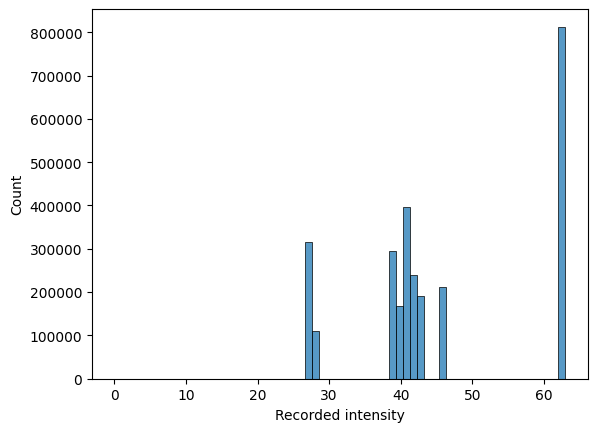
\includegraphics[width=\textwidth]{../images/03a_lysva_dataset-fig-intensity-with-example-output-1.png}
}
\subcaption{\label{fig-intensity-with-example-1}Distribution of
intensity over all points in the Lysva dataset.}
\end{minipage}
\begin{minipage}{0.50\linewidth}
\centering{
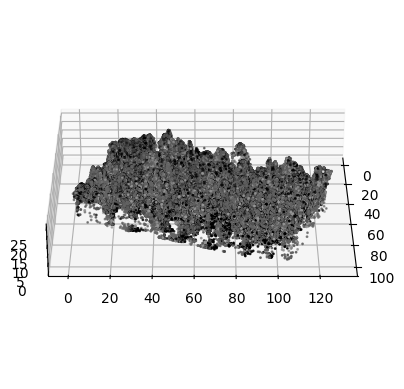
\includegraphics[width=\textwidth]{../images/03a_lysva_dataset-fig-intensity-with-example-output-2.png}
}
\subcaption{\label{fig-intensity-with-example-2}A point cloud of plot 10
with points colored by intensity.}
\end{minipage}
\caption{\label{fig-intensity-with-example}An example of the
unreliability of the intensity attribute.}
\end{figure}

Some sensors do provide more consistent values.
However, relying on intensity-based features limits the applicability of developed models and methods, as any such model would surely fail on data like this.

\subsubsection{Comparison to other datasets}

Our dataset is in many ways similar to the NewFor benchmark \cite{eysnAlpineITDBenchmark2015}.
It serves the same purpose and also offers overlapping field survey ground plots and \gls{uav} \gls{lidar} point clouds.
There are, however, many notable differences.
The NewFor benchmark covers much more diverse regions, including ground plots from France, Italy, Switzerland, Austria, and Slovenia, while all our data comes from the same area.
The tree species covered by the datasets are also different: both contain spruce and fir, but the NewFor data also has beech, Scots pine, larch, sycamore, and poplar, while ours also has birch, aspen, tilia, alder, and willow.
Our dataset has more than twice as many individual trees as the Alpine benchmark, and the forest is denser and more complex, making it more complicated to detect trees in.
Our data contains very mild terrain variations, while the slopes of the terrain in Alpine data are very steep, which plays a role during height normalization, since subtraction of steep terrain introduces artificial slope to the points in the canopy, changing the overall shape of the tree.
Our dataset has an additional information source – an \gls{rgb} orthophoto that allows development of algorithms that fuse multimodal data, which, we believe, is a key to success in such complex environments.
Our dataset has species labels for every surveyed tree, but only partial coverage of tree heights and no timber volume information at all.

Another similar dataset is the NeonTreeEvaluation Benchmark \cite{weinsteinDataNeonTreeEvaluationBenchmark2022}, which offers bounding box annotation for tree detection across a wide range of different forest types.
It offers coregistered \gls{rgb}, \gls{lidar}, and hyperspectral images over 31,000 individual trees.
The main difference in the reference data between the NeonTreeEvaluation Benchmark and our dataset is the source: our data comes from a field inventory and thus has additional tree information that can be used in downstream tasks, such as species classification or timber volume prediction, while the NeonTreeEvaluation Benchmark annotations are created from the \gls{rgb} photo and thus only offer the positions and sized of trees.

Another dataset is the IDTReeS 2020 Competition Data \cite{gravesIDTReeS2020Competition2020} aimed to develop algorithms for delineation and species classification of individual tree crowns in \gls{rgb}, \gls{lidar}, and hyperspectral data.
It offers bounding box annotations for 1200 individual trees covered by \gls{rgb}, \gls{lidar}, and hyperspectral images in 3 national forests in the USA.
Similarly, the source of the data is annotation of images, not a field inventory.

There are also datasets available that do not have \gls{lidar} point cloud coverage, or use terrestrial \gls{lidar} instead of \gls{uav} \gls{lidar}, or use photogrammetric point clouds instead of \gls{lidar} point clouds.
We do not mention them here because we specifically focus on \gls{uav} \gls{lidar}.

\section{Individual tree point clouds dataset}\label{sec-individual-trees-dataset}

The main dataset used for training the models is a collection of point clouds of individual trees, sometimes referred to in this text as tree clouds, extracted manually from larger \gls{uav} \gls{lidar} point clouds.
The dataset is released into open access, and was originally presented in \citep{dubrovinExplorationPropertiesPoint2024}, although it has been expanded since and now contains twice as many individual trees.
It consists of 394 trees, 192 of which are extracted from the previously described Lysva survey, and 202 from other surveys in Perm Krai.
The distinction between the parts is important because the Lysva dataset has \gls{rgb} orthophoto coverage, making it possible to infuse the tree clouds with orthophoto-based features.
Thus, for training the tree segmentation networks that rely on these features, the effective size of the dataset is 192 tree clouds, as only the former part is used.
However, the whole dataset is used for training regression and classification models that process segmented trees.

Figure~\ref{fig-individual-trees-species-distribution} shows the distribution of species in the individual tree point clouds dataset.
The split between coniferous and deciduous trees is almost even: there are 202 coniferous and 193 deciduous trees.
There are seven species in total: spruce, birch, aspen, pine, fir, alder, and tilia, with most focus on 4 most important species listed first.
Note the presence of pine trees, which are not present in the Lysva field inventory data, and the absence of willow trees.
All the pine trees are from other field surveys.
Willows are skipped intentionally, since they are of little interest in terms of timber harvesting: they are considered low quality, and their ripening cycle is mismatched with main timber species – when the overall plot is ready to be harvested, the willows are already rotten.

\begin{figure}
\centering{
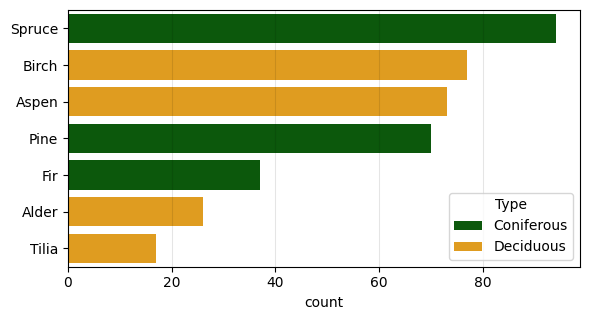
\includegraphics[width=\textwidth]{../images/03b_individual_trees-fig-individual-trees-species-distribution-output-1.png}
}
\caption[Distribution of tree species in the individual trees dataset]{\label{fig-individual-trees-species-distribution}Distribution
of tree species in the individual trees dataset. It contains 394 point
clouds of individual trees: 201 coniferous and 193 deciduous. Note the
presence of pine trees, as there are no pine trees in the Lysva field
inventory -- all of the pines come from other field surveys.}
\end{figure}


Figure~\ref{fig-individual-trees-visualization} is a visualization of the data.
It shows a random tree of every species as a 2D scatter plot and a single spruce as a 3D scatter plot with points colored by height.
Because the observations are made from above, many trees have the highest concentrations of points at the top of their canopy and a very limited number of points along the trunk.
Additionally, slight slopes of the terrain manifest as artificial tilt in some of the trees because of the height normalization of the original point cloud.

\begin{figure}
\begin{minipage}{0.7\linewidth}
\centering{
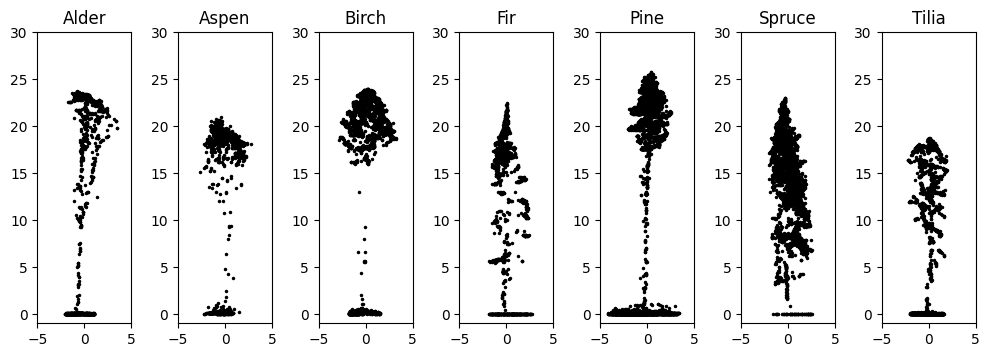
\includegraphics[width=\textwidth]{../images/03b_individual_trees-fig-individual-trees-visualization-output-1.png}
}
\subcaption{\label{fig-individual-trees-visualization-1}Cross-sections
of random trees of every species (ignoring the Y dimension).}
\end{minipage}
\begin{minipage}{0.29\linewidth}
\centering{
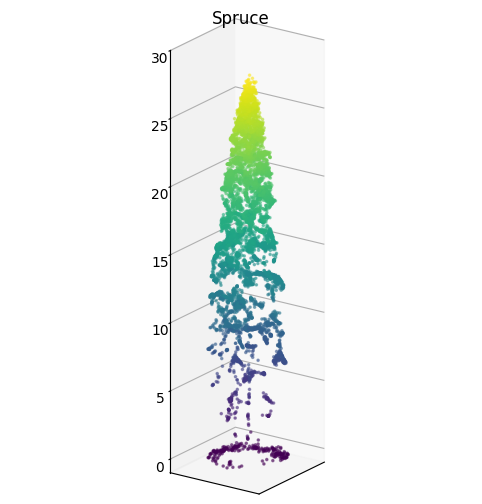
\includegraphics[width=\textwidth]{../images/03b_individual_trees-fig-individual-trees-visualization-output-2.png}
}
\subcaption{\label{fig-individual-trees-visualization-2}A spruce in 3D.}
\end{minipage}
\caption[Visualizations of the individual tree point clouds in the dataset.]{\label{fig-individual-trees-visualization}Visualizations of the
individual tree point clouds in the dataset. Most of the tree clouds are
top-heavy because of the observation from above, and some are
artificially tilted because of slight terrain slopes and height
normalization. The ground points are present.}
\end{figure}

An important note is that the extracted trees were not chosen for extraction randomly but were selected by humans based on whether it was possible and relatively easy to separate from the surrounding trees.
So there is a selection bias in there favoring the trees that are easily separable, standing outside of large dense clusters.
Because of that the trees do not exactly represent what a tree closely surrounded by other trees is like in a point cloud.
It is especially apparent in very pronounced trunks of all the visualized trees.
In a dense forest, such as the one visualized in Figure~\ref{fig-lysva-canopy-structure}, there is hardly ever enough penetration for such detailed trunk coverage.
In fact, as mentioned in the literature review, good coverage of trunks is an immensely useful feature of terrestrial \gls{lidar} surveys, which consistently show very good results using algorithm that segment trees from the trunk up.

\section{Synthetic forests generated from individual trees}\label{sec-synthetic-forest-dataset}

To train tree segmentation models, training data where every point is assigned to an individual tree is required.
Data like that are very labor-intensive to label.
An alternative way to create such data is by generating it from a set of tree clouds, as the per point labels arise naturally in this case.
I used the dataset of individual tree point clouds described in the previous section to generate a synthetic forest to train a tree segmentation PointNet++.

Synthetic forest is generated in patches of set height and width by sampling individual trees from the full set and placing them from left to right, until the set width is extended, then from bottom to top, until the set height is extended.
A height threshold is applied to each tree before placing it to remove ground points and non-tree reflections.
This results in patches that are slightly bigger than the set size, but that can be cropped into the exact size.
This has an added benefit of mimicking cutoff trees at the edges of the patch that are inevitable when the model is applied in a sliding window.
The trees can be sampled with or without replacement, but since a set of augmentations described in Section~\ref{sec-augmentations} is applied to each tree individually, exact same tree never occurs in the patch fed to the model even when sampling with replacement.
When trees are placed, their planar bounding boxes are tracked to avoid overlap.
However, since some overlap might, in fact, be desired to better represent actual forests, a parameter that controls the amount of overlap is added to the dataset generation process.
Each tree is also assigned a label, which simply tracks its ordinal number in the patch.
An example of a 20 by 20 meter synthetic forest patch with 0.75 meter overlap and 2 meter height threshold is shown in Figure~\ref{fig-synthetic-forest-patch-example} from two different perspectives and using two color schemes: the label, i.e. the ordinal ID of the tree within a patch, and \gls{rgb} color sampled from the orthophoto.

\begin{figure}
\centering{
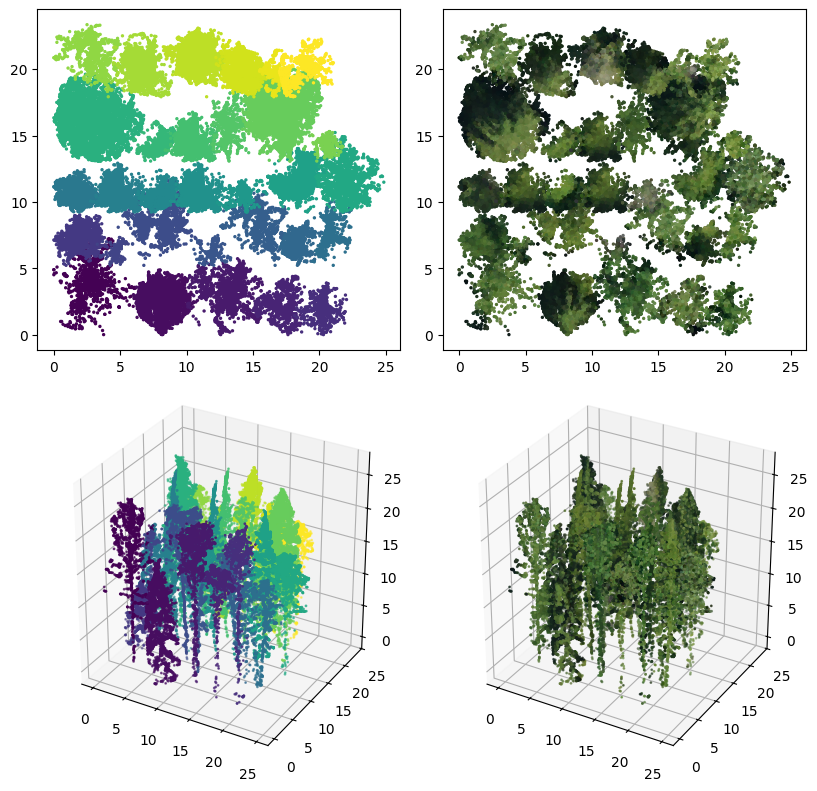
\includegraphics[width=\textwidth]{../images/03c_synthetic_forest-fig-synthetic-forest-patch-example-output-1.png}
}
\caption[Visualisation of a synthetic forest patch used for
training]{\label{fig-synthetic-forest-patch-example}A visualization of a
synthetic forest patch used for training the tree segmentation network.
Patch width and height are set to 20 meters, overlap is set to 0.75.
\textbf{Top:} Top-down view of the patch. \textbf{Bottom:} 3D view of
the same patch. \textbf{Left:} Points colored by label: unique tree ID
within the patch. \textbf{Right:} Points colored by RGB color sampled
from the orthophoto.}
\end{figure}

For comparison, a patch of the same size from a real point cloud over one of the plots of the Lysva survey is shown in Figure~\ref{fig-lysva-plot-window-example}.

\begin{figure}
\centering{
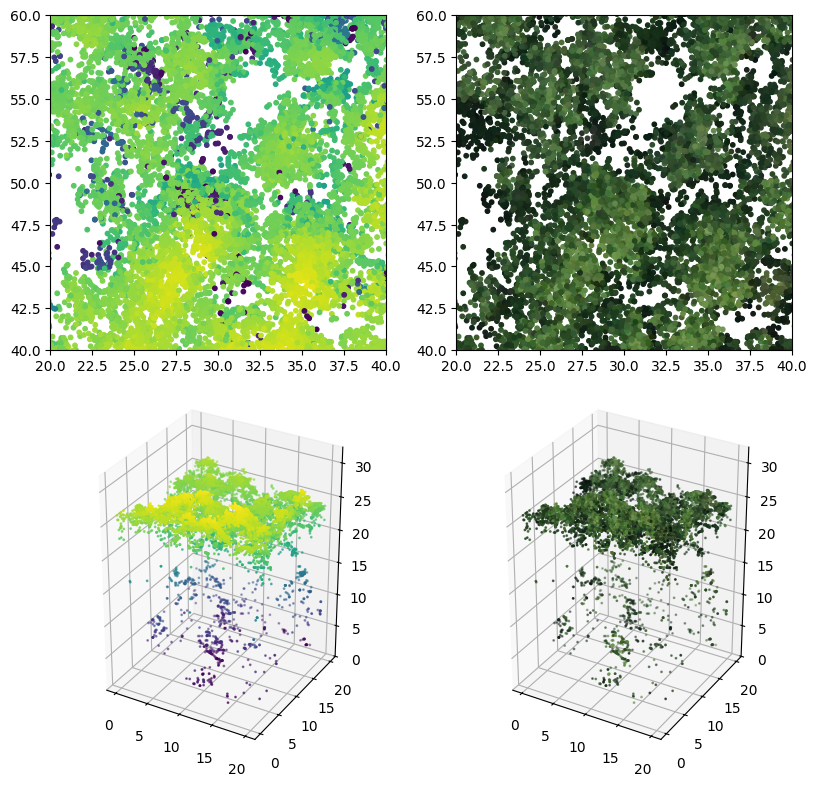
\includegraphics[width=\textwidth]{../images/03c_synthetic_forest-fig-lysva-plot-window-example-output-1.png}
}
\caption[Visualisation of a patch of a real forest.]{\label{fig-lysva-plot-window-example}A piece of the Lysva
LiDAR point cloud over plot 10 in within a 20 by 20 meter window.
\textbf{Top:} Top-down view. \textbf{Bottom:} The same patch in 3D view.
\textbf{Left:} Points colored by height. \textbf{Right:} Points colored
by RGB color sampled from the orthophoto.}
\end{figure}

An alternative approach to creating patches of synthetic forest can be to use a fixed number of trees instead of fixed patch size.
However, it poorly correlates with how the final model will be applied: in windows of fixed size, not windows with varying size but fixed number of trees.
And size of the patch the model sees is important because the scale is normalized, and using a different patch sizes changes the scaled coordinates and confuses the model that learned to rely on them.

Enriching point clouds using only color information from \gls{rgb} orthophotos provides limited utility because it adds only local information to the points.
As was mentioned in the introduction, one of the aspects of the complementary nature of the two data sources is that images provide continuous representations and capture textures.
To enrich the image features with context, they can be preprocessed with feature extractors that encode context into pixel values and thus provide more information for the segmentation network.
The feature extractors can be simple algorithms or specialized convolutional network feature extractors.
For the same reason a simple PointNet++ is used as the architecture for the tree segmentation network, a simple collection of multi-scale features are used as orthophoto features, including intensity, edge, and texture features, extracted from the orthophotos using the \texttt{scikit-image} Python package.
The features are calculated on different scales by applying Gaussian smoothing with varying parameters before calculation.
Figure~\ref{fig-basic-features-small} shows example features from every mentioned group on a very fine scale.
The top left image is the original orthophoto of plot 10 from the Lysva survey, the top right image is the intensity calculated from it, and bottom images are examples of an edge feature and a texture feature.
The same features but on a coarser scale are shown in Figure~\ref{fig-basic-features-large}.

\begin{figure}
\centering{
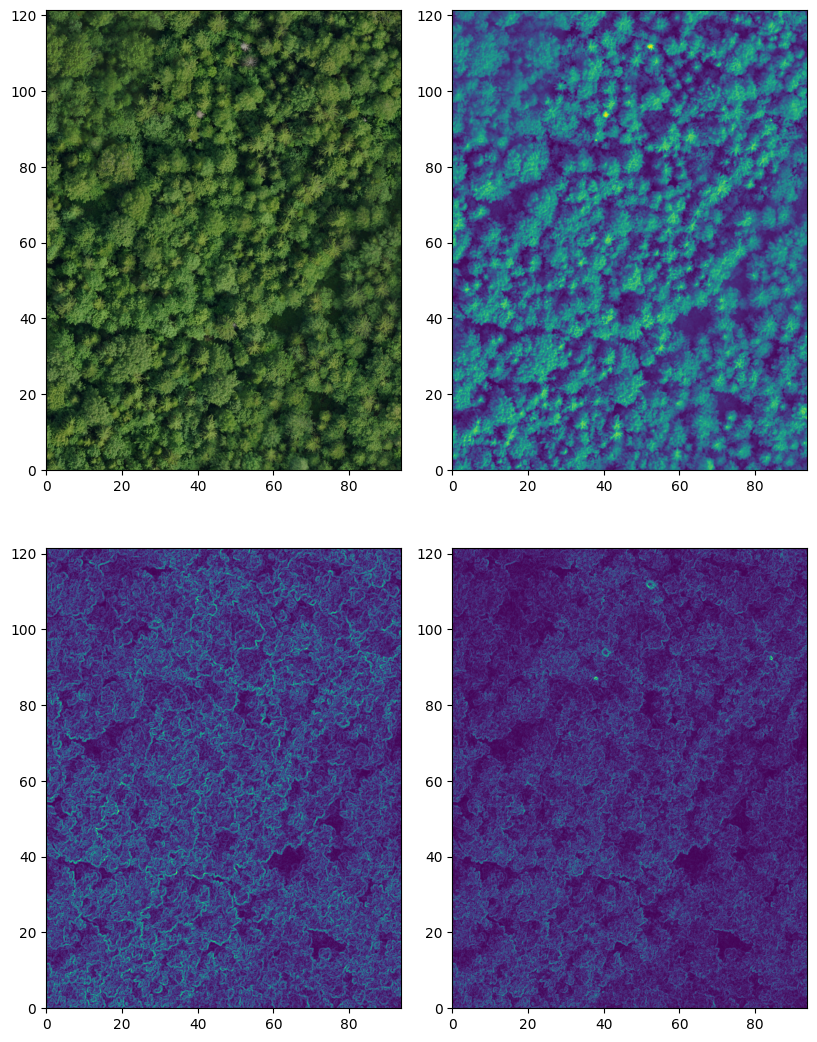
\includegraphics[width=\textwidth]{../images/03c_synthetic_forest-fig-basic-features-small-output-1.png}
}
\caption[Visualisation of basic orthophoto-based features (small
scale)]{\label{fig-basic-features-small}Basic orthophoto-based features
used (on a single scale with sigma=1, actual features are across
multiple increasing scales). \textbf{Top left}: The original orthophoto
for plot 10. \textbf{Top right}: Intensity feature. \textbf{Bottom
left}: Edges feature. \textbf{Bottom right}: Texture feature.}
\end{figure}

\begin{figure}
\centering{
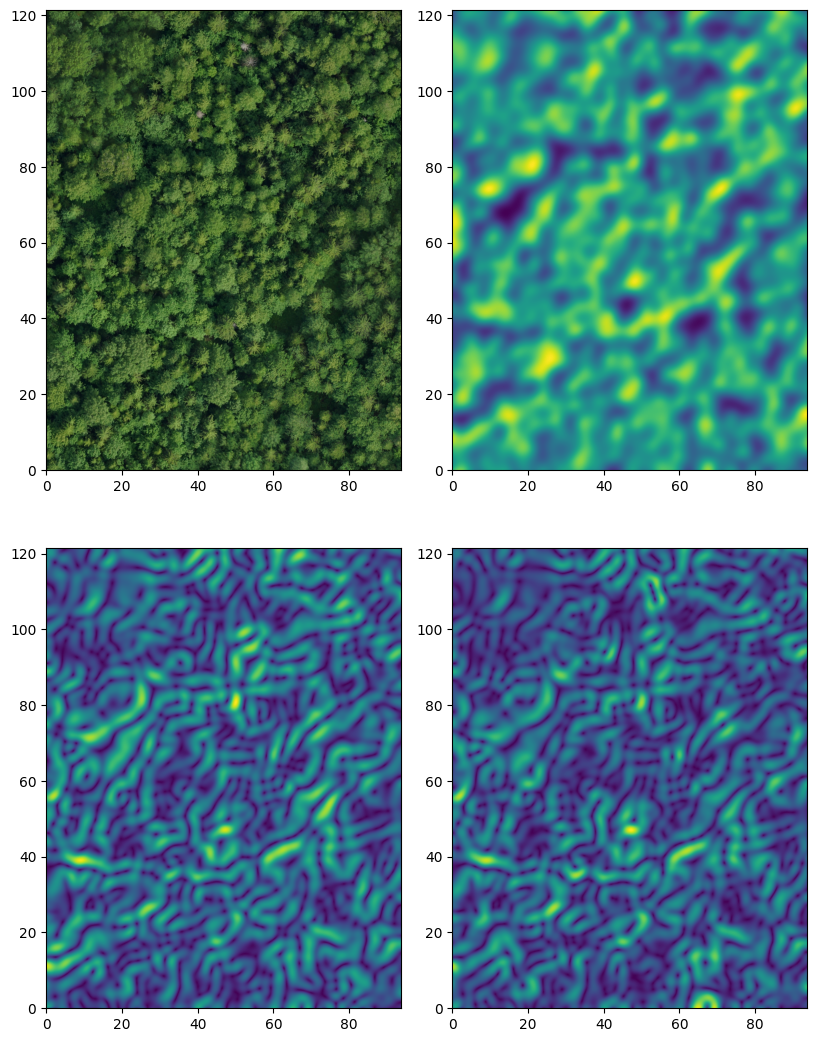
\includegraphics[width=\textwidth]{../images/03c_synthetic_forest-fig-basic-features-large-output-1.png}
}
\caption[Visualisation of basic orthophoto-based features (large
scale)]{\label{fig-basic-features-large}Basic orthophoto-based features
used (on a single scale with sigma=16, actual features are across
multiple increasing scales). \textbf{Top left}: The original orthophoto
for plot 10. \textbf{Top right}: Intensity feature. \textbf{Bottom
left}: Edges feature. \textbf{Bottom right}: Texture feature.}
\end{figure}

It is worth mentioning that using synthetic data for training comes with potential biases that are important to keep in mind.
The biases present in the source dataset can easily become exaggerated.
In this case, the selection bias mentioned in Section~\ref{sec-individual-trees-dataset} is the main potential culprit.
The limited size of the source dataset also limits the variability of the examples, which can easily lead to complex overfitting.
In this case, the range of shapes of the trees within each species is small, making it hard to generalize well.
Moreover, different species will most likely have different accuracies associated with them.
Models trained entirely on synthetic datasets are also a lot harder to properly evaluate.
These drawbacks are partially addressed by carefully choosing the augmentations for the training procedure, but they cannot be completely circumvented.

\section{Training tree segmentation neural networks}

The architecture chosen to serve as the tree segmentation network is the PointNet++ \citep{qiPointNetPlusPlus2017}, described in detail in Section~\ref{sec-ml-dl}.
It is a relatively simple architecture, and further potential quality improvements might be achieved by using more modern and advanced architectures instead.
However, the main goal of this thesis was to develop and verify an overall framework, and thus the choice was set on a model that is simple to implement and work with to allow easy experimentation with other parts of the proposed system.

The architecture of the used PointNet++ is similar to the segmentation architecture shown in Figure~\ref{fig-pointnet2-architecture}.
The main differences from the shown architecture are the use of one more stacked set abstraction layer to make the network deeper, and the use of a regression head that predicts a continuous value for each point instead of a classification head that predicts per-point class scores, since the model needs to assign a unique ID to every tree in the patch.
The three stacked set abstraction layers have the proportions of points sampled set to 0.75, 0.5, and 0.5, and neighborhood radii for feature aggregation set to 0.1, 0.2, and 0.4.
Note that the scale of the input is normalized (see next subsection for details), so the radii are not in meters.
The model has 30 million trainable parameters.

\subsection{Coordinate and feature normalization}

It's a well established practice to scale the inputs to neural networks that is known to improve the speed and accuracy of gradient descent convergence \citep{bishop2006pattern}.
Before going through the network, a set of augmentations and transformations is applied to each synthetic forest patch.
The augmentations are described in detail with visualized examples in Section~\ref{sec-augmentations}.
The transformations include scale and feature normalization – the coordinates are centered and normalized to the interval $(-1, 1)$ and the features are normalized to the interval $(-1, 1)$ without centering.

\subsection{Data augmentation}\label{sec-augmentations}

The primary objective of data augmentation is to enhance the quantity, quality, and variety of data used for training \citep{mumuniDataAugmentationComprehensive2022}.
This is especially important when the sizes of the available datasets are limited, like in the case of the individual trees data that is the base of the synthetic forest datasets.
Carefully selected augmentations allow increasing the effective dataset size.
However, it is important to pay attention that the chosen augmentations keep the transformed examples semantically equivalent to the original.
A readily understandable example of a bad augmentation in the task of digit classification, which is often used as the "hello world" of deep learning with the MNIST dataset of handwritten digits \citep{deng2012mnist}, is a vertical flip, as most digits lose meaning when upside down.
A flip is also a bad augmentation example for a synthetic forest patch described in Section~\ref{sec-synthetic-forest-dataset}, as it changes the order of the trees within a patch, thus breaking the labels that are assumed to increase in a specific pattern.

In the scenario when the data for is created by combining several smaller inputs, there is a possibility of applying augmentations on two different scales.
The most simple approach is to treat a synthetic forest patch as a whole and apply augmentations directly to it.
However, it is also possible to apply per-tree augmentations, effectively increasing the size of the underlying tree set from which synthetic forest patches constructed.
Only the latter kind are used for training the tree segmentation network.

The first transformation that changes the shape but does not affect any semantics for an individual tree is a random rotation around the vertical axis.
A tree remains completely the same when rotated, but the coordinates of all points change.
Figure~\ref{fig-random-rotate-effect} shows the effect of applying random rotation transformation of different magnitudes to a single aspen tree.
For visualization purposes, the rotation is forced to apply with full magnitude for every parameter.
During training, the angle is uniformly sampled from the specified range.
For the final tree segmentation model, the range is set to $[-180, 180]$ degrees, as no amount of rotation breaks the semantics.

\begin{figure}
\centering{
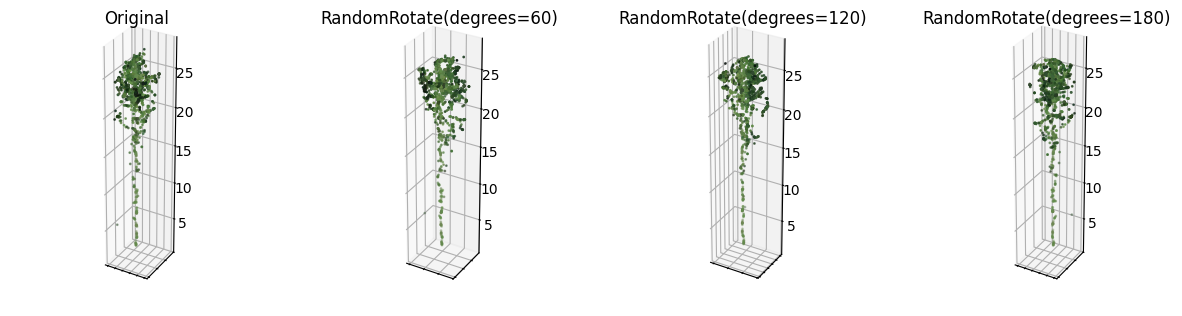
\includegraphics[width=\textwidth]{../images/03d_augmentations-fig-random-rotate-effect-output-1.png}
}
\caption[Visualization of the random rotation around Z axis augmentation on a single aspen tree.]{\label{fig-random-rotate-effect}Visualization of the random
rotation around Z axis augmentation on a single aspen tree. The effect
is forced to happen with full amplitude for visualization purposes,
during training a rotation angle is uniformly sampled from a set range.}
\end{figure}%

Another transformation that keeps the tree the same but changes the coordinates of the points is random scaling.
It simply multiplies the coordinates by a scaling factor, making the tree larger or smaller in all directions.
Unlike random rotation around the vertical axis, however, the range needs to be chosen much more carefully, as there is a possibility of making unrealistically large or small trees that would confuse the model during training.
Figure~\ref{fig-random-scale-effect} shows the effect of applying random scale transformation to a single aspen tree.
Again, for purposes of visualization, the scale is forced to apply with full magnitude.
During training, the scale is uniformly sampled from the specified range.
For the final tree segmentation model, the range is set to $[0.8, 1.2]$.

\begin{figure}
\centering{
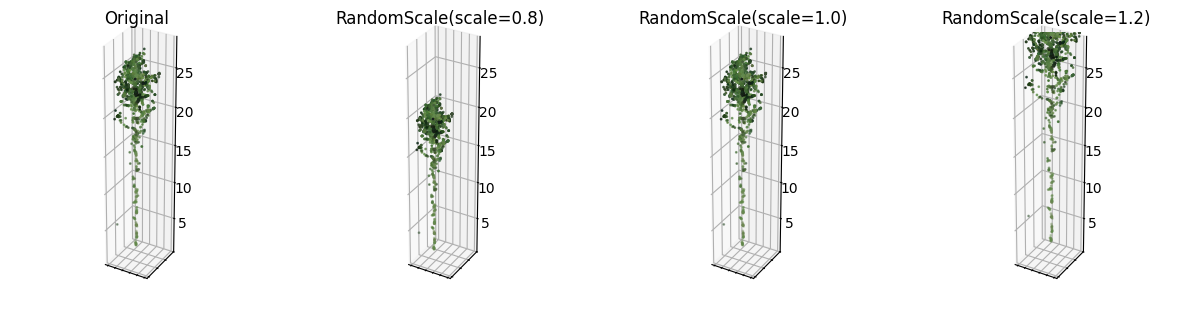
\includegraphics[width=\textwidth]{../images/03d_augmentations-fig-random-scale-effect-output-1.png}
}
\caption[Visualization of the random scale augmentation on a single aspen tree.]{\label{fig-random-scale-effect}Visualization of the random
scale augmentation on a single aspen tree. The effect is forced to
happen with full amplitude for visualization purposes, during training a
scale factor is uniformly sampled from a set range.}
\end{figure}

Another way to change the positions is to slightly translate each point for a random distance in a random direction.
That transformation is commonly referred to as random jitter.
Since \gls{lidar} sensors have limited spatial accuracy, introducing random translations within the accuracy range should not have any effect on the result of tree segmentation.
Going further, small translations even outside the accuracy range make sense, since they have very limited effect on the overall shape of the tree.
Figure~\ref{fig-random-jitter-effect} shows this effect on a single aspen tree.
The amount of translation is uniformly sampled independently for each point from a set range.
Note that the random jitter augmentation is applied before the scale normalization.
It matters because the augmentation's only parameter is the translation range, which depends on the scale.
The parameters on the figure are thus in the original coordinate units – meters.
Note how the shape of the tree almost does not change when the maximum range is set to 20 centimeters, and starts to become fuzzy and loose shape at 1 meter and higher.
For the final tree segmentation model, the maximum translation is set to 30 centimeters.

\begin{figure}
\centering{
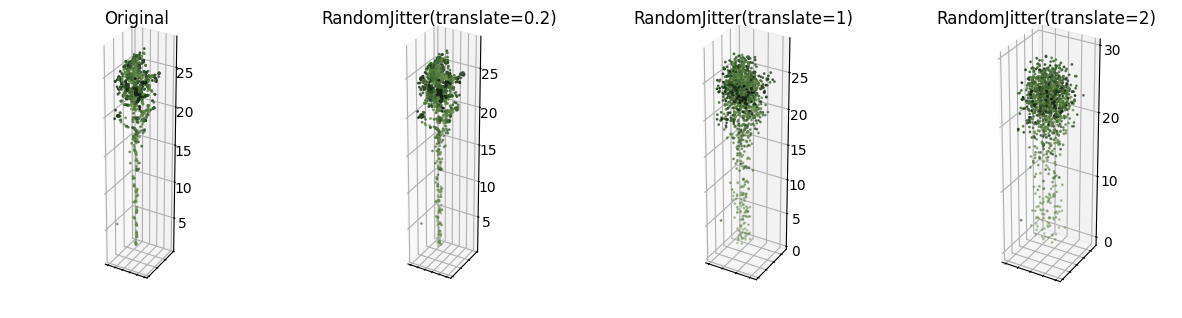
\includegraphics[width=\textwidth]{../images/03d_augmentations-fig-random-jitter-effect-output-1.png}
}
\caption[Visualization of the random jitter augmentation on a single aspen tree.]{\label{fig-random-jitter-effect}Visualization of the random
jitter augmentation on a single aspen tree. The translation magnitude is
uniformly sampled from a set range for every point.}
\end{figure}

Another useful effect augmentations can provide is to make synthetic data look more like real data.
As was mentioned in Section~\ref{sec-individual-trees-dataset}, there is a selection bias in the dataset of individual trees: the trees that are easiest to manually separate are exponentially more likely to end up in the data.
As such, the tree clouds in the individual tree dataset are significantly different from trees of the same species with similar sizes and shapes, but standing in dense clusters.
One of the most important differences is that almost all the tree clouds have trunks, while in actual forest, dense canopy cover blocks most pulses and the trunk representation is very poor.
One way to mitigate that issue is to apply a height-dependent dropout function to each tree cloud.
For that purpose a probability threshold function that is around zero for the highest points of the tree and quickly ramps up to almost one for the lowest points is needed.
An example function that satisfies these criteria is a modified sigmoid:

$$
\text{threshold}(z) = \big[1 + e^{z \times \text{scale} + \text{shift}}\big]^{-1},
$$

where $z$ is the height normalized to $[0, 1]$ and reversed by subtraction from 1, $\text{scale}$ and $\text{shift}$ are hyperparameters that control the shape of the curve.
Changing $\text{scale}$ controls how steep is the climb from 0 to 1: the larger, the steeper.
Changing $\text{shift}$ controls the position of the climb: the larger, the lower.
Figure~\ref{fig-height-dropout} shows an example of applying such dropout function to a single aspen tree, and Figure~\ref{fig-height-dropout-aggressive} show the same tree with more aggressive parameters, resulting in much more points being dropped from the tree cloud.

\begin{figure}
\centering{
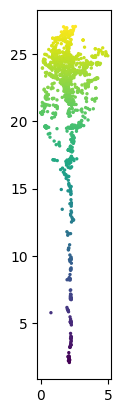
\includegraphics[width=\textwidth]{../images/03d_augmentations-fig-height-dropout-output-1.png}
}
\caption[Effect of the height-dependent modified sigmoid dropout on a single aspen tree.]{\label{fig-height-dropout}Effect of the height-dependent
modified sigmoid dropout on a single aspen tree. Scale is set to 8,
shift is set to 3. \textbf{a)} A single aspen tree with points colored
by height. \textbf{b)} Height-dependent probability of dropout (a
modified sigmoid). \textbf{c)} The same aspen with points colored by
probability of dropout. \textbf{d)} The same aspen with points that will
be dropped marked red. \textbf{e)} The same aspen after the dropout is
appleid with point colored by height.}
\end{figure}

\begin{figure}
\centering{
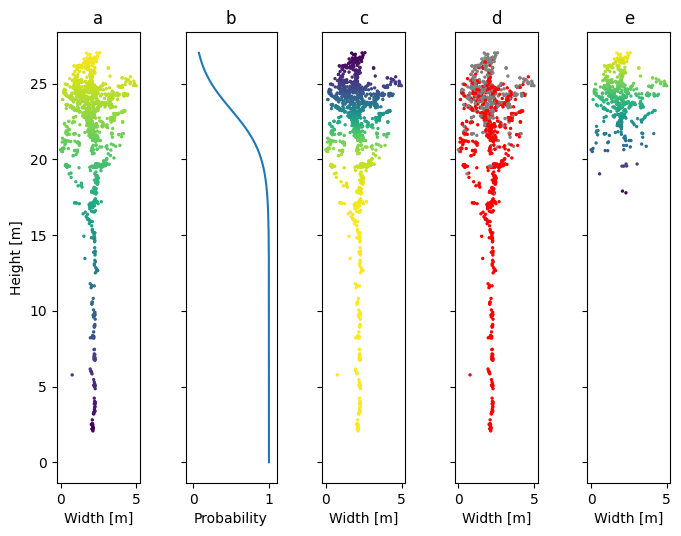
\includegraphics[width=\textwidth]{../images/03d_augmentations-fig-height-dropout-aggressive-output-1.png}
}
\caption[Effect of a stronger height-dependent modified sigmoid dropout on a single aspen tree.]{\label{fig-height-dropout-aggressive}Same as
Figure~\ref{fig-height-dropout}, but with a more aggressive dropout
threshold function. Scale is set to 18, shift is set to 2.5.}
\end{figure}

All the augmentation are applied on the fly right before the examples are loaded into GPU memory and passed through the network.

\subsection{Other training parameters}\label{sec-other-training-params}

Mean absolute error is used as a loss function.
Some experiments have shown improvements when using a custom loss function that modifies the mean absolute error loss by weighting it reversely proportional to the distance of the tree centroid.
The idea of the modification is to make the network focus more on points closer to the center of each tree, as these points are much less likely to be overlapping with the crowns of adjacent trees.

The batch size is limited by the available GPU device memory, and in the described setup competes for memory space with the synthetic forest patch dimensions used in the training dataset.
The preference is given to the size of the patch, so the batch size is set to 1, but is compensated for by using gradient accumulation steps – updates to the model parameters are made after the gradient is accumulated for a set number of iterations.
This slows down the training, but enables usage of larger batches when there is not enough memory to fit them, making the training procedure overall more stable.

Early stopping \citep{precheltAutomaticEarlyStopping1998} is set up to terminate training early if there is no improvement in average validation loss in a set number of epochs.
This makes sure that valuable GPU time is not wasted on continuing training models that are likely to have started overfitting.

Model checkpointing is set up as well.
After each training epoch, when the average validation loss and accuracy are calculated, the model state is saved to disk if it's current accuracy is better than the last saved one, where accuracy is the proportion of points for which the rounded integer label is correct.
This makes sure that the best performing model can always be recovered, even if the training process was run for too long and the latest model is not the best one.

The learning rate schedule is set to follow a fast linear warm up and slow linear decay.
Learning rate is set to ramp up from 0.001 to 0.01 in a span of 2 epochs, and then decay back to 0.001 in a span of 30 epochs.
Adam optimizer is used \citep{kingmaAdamMethodStochastic2014}.

Training was performed on an NVIDIA A100 GPU with 80 Gb of memory.
Inference, depending on the point density of the input, might work even on a much smaller GPU like Tesla T4 with 16 Gb of memory.
GPUs of this size are available with limits on usage for free on services like Google Colab and Kaggle.

\subsection{On implementation of PointNet++}

As mentioned in the introduction, the deep learning code, including the code for PointNet++, is implemented using the PyTorch Geometric library designed for writing and training graph neural networks.
This makes the implementation not exactly the same as described in the PointNet papers.
The main ideas, namely local feature learning in a k-nearest neighbors neighborhood and max pooling for permutation-invariant aggregation, are there.
Input transform and feature transform networks are not defined explicitly, but networks that process features learn to perform a similar function.

\section{Training segmented trees processing models}\label{sec-training-tree-processors}

To predict per-tree forest attributes from a segmented point cloud, a set of specialized regression and classification models is trained on the tree clouds.
These specialized models are classic machine learning models that operate on most common metrics described in the literature overview chapter.
As mentioned in the literature overview, common features used for machine learning on point clouds are based on the eigenvalues of the covariance matrix of the point coordinates, calculated either for an entire cloud, or per-point in a neighborhood around it.
These features include linearity, planarity, scatter, that aim to indicate the presence of linear, planar, or volumetric structures, and also omnivariance, anisotropy, eigentropy, the sum of eigenvalues, and curvature.
The features are defined as follows, with eigenvalues sorted in descending order such that $\lambda_1 \ge \lambda_2 \ge \lambda_3$:

$$
\begin{aligned}
\text{linearity} &= \frac{\lambda_1 - \lambda_2}{\lambda_1} \\
\text{planarity} &= \frac{\lambda_2 - \lambda_3}{\lambda_1} \\
\text{scatter} &= \frac{\lambda_3}{\lambda_1}  \\
\text{omnivariance} &= \sqrt[3]{\lambda_1\lambda_2\lambda_3} \\
\text{anisotropy} &= \frac{\lambda_1 - \lambda_3}{\lambda_1} \\
\text{eigentropy} &= -\sum_{i=1}^{3} \lambda_i \ln(\lambda_i) \\
\text{sum of eigenvalues} &= \lambda_1 + \lambda_2 + \lambda_3 \\
\text{curvature} &= \frac{\lambda_3}{\lambda_1 + \lambda_2 + \lambda_3} \\
\end{aligned}
$$

Another common set of features, especially popular in forestry applications, are various statistics that describe the height distribution of points within the neighborhood or the cloud.
They include maximum and average height, standard deviation, kurtosis, skew, and entropy of the height distribution, percentage of points above the mean and each of the deciles of height and the deciles of height themselves.
The features are calculated for the entire tree cloud, effectively reducing each tree to a collection of metrics, resulting in a tabular dataset.
In this form, the dataset is used to train the models.

In \citet{dubrovinExplorationPropertiesPoint2024}, we propose a way to help build intuition into the meaning of some of the less obvious features by visualizing individual trees on a different end of the range of the feature's values.
Figure~\ref{fig-feature-ranges} shows is an example of such visualization, showing the effect of the shape of spruce on omnivariance and the effect of the shape of aspen on percent of points above mean height.
Note the presence of ground points, which are filtered out before calculating features for the models.

\begin{figure}
\centering{
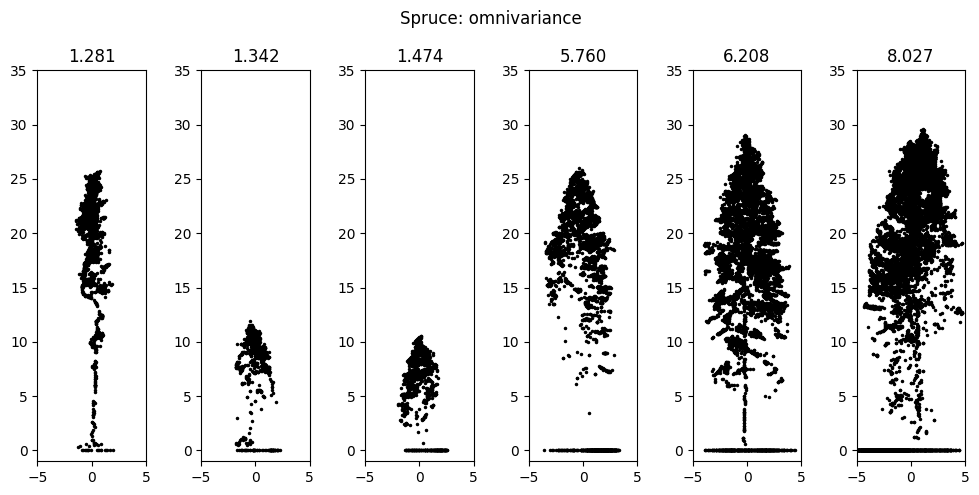
\includegraphics[width=\textwidth]{../images/fig-feature-ranges-output-1.png}
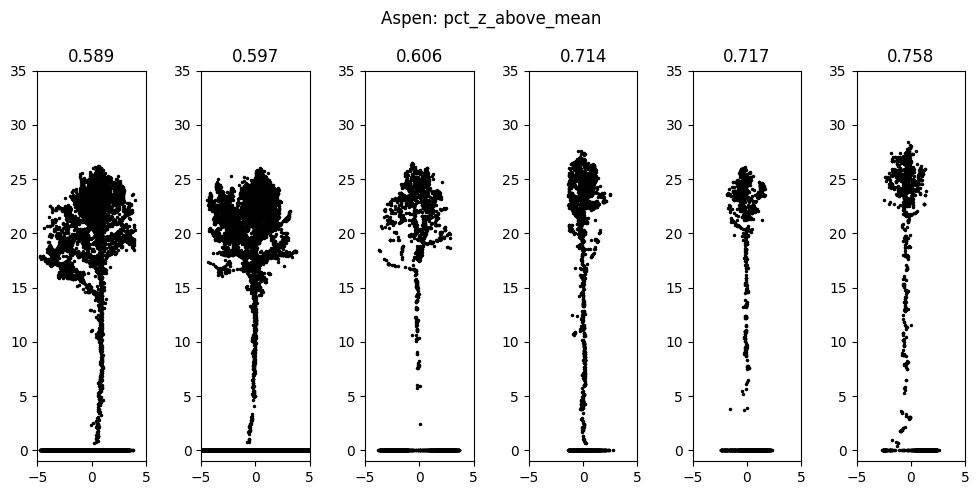
\includegraphics[width=\textwidth]{../images/fig-feature-ranges-output-2.png}
}
\caption[Visualizations of tree shapes at different ends of feature value ranges.]{\label{fig-feature-ranges}Visualizations of how values of
commonly used features calculated for the whole tree cloud map to the
shapes of individual trees. \textbf{Top}: Effect of the shape of spruce
on omnivariance. \textbf{Bottom}: Effect of on the shape of aspen on
percent of points higher than mean height. Figure reused from Dubrovin
and Fortin (2024). Note the presence of ground points, which are
filtered out before calculating features for the models.}
\end{figure}

The feature set is thinned by using sequential feature selection: a greedy approach that selects the best feature according to 5-fold cross-validation accuracy on every iteration until a set number of features is selected.
The models are trained on 20 best features selected this way.

To make the trees more closely resemble the trees standing in dense clusters, the same height-dependent dropout function that is used for augmenting synthetic forests is used.
This dropout, together with a small amount of random jitter, is also used to create additional samples for training the models, as the original dataset size is very small.
Great care is taken to only create additional samples within the training set, to avoid any data leakage.
Every training set sample is repeated 3 times with random jitter with maximum amplitude of 20 cm and a dropout applied.

Two models are used as proof of concept for the proposed framework: a classifier that predicts the tree species, and a regressor that estimates a tree's diameter at breast height.
Random Forest models are used in both cases.
The number of trees is set to 200.
For the classification model, class weights are assigned to every example that are inversely proportional to the class frequency in the data during model fitting.

\section{Matching detected trees to ground truth}\label{sec-matching-algorithm}

To evaluate the results of any tree detection system against field inventory data, an automated and deterministic method for matching detected tree candidates to the ground truth trees is needed.
It should determine which ground truth trees, if any, the detected candidates correspond to.
It should also classify both the trees and the candidates as either a true positive, meaning that the ground truth tree was successfully detected, a false negative, meaning that a ground truth tree was not detected, or a false positive, meaning a tree was detected when there is none.

I use the same matching procedure that is described and implemented in \citet{dubrovinOpenDatasetIndividual2024}.
It considers the locations and heights of the trees, and falls back to using only locations when the height is not available for the ground truth tree.
It is parametrized by the maximum allowed 2D distance and the maximum height difference between a detected and a ground truth tree to consider them a match.
First, it constructs a distance matrix between the ground truth tree locations and the detected candidates and filters out the pairs for which the distance is larger than the allowed maximum.
It then iterates over the remaining pairs in the order of increasing distance, and marks the pairs with suitable heights in which both trees are not yet assigned a class as a true positive.
The pairs in which one of the trees is already assigned a class are marked as either a false positive or a false negative, and the pairs in which both trees are assigned a class are skipped.
Finally, it marks all unmatched ground truth trees as false negatives, and all unmatched candidate trees as false positives.

Based on the results of the matching algorithm, a set of metrics that are often used to evaluate the results of tree detection can be calculated.
The same metrics are usually used for evaluation in classification problems and thus are well-known.
The first commonly used metric is recall, which is the proportion of the ground truth trees that were detected.
The second metric is precision, which is the proportion of candidates that are correct.
Both are important, and describe a detection system from different perspectives.
To combine them into a single metric, $F_1$-score is often used, which is the harmonic mean of precision and recall that provide a balanced measure of the system performance.
The formulas for the metrics are as follows:

$$
\text{recall} =
\frac{N_{\text{true positives}}}{N_\text{trees}} =
\frac{N_{\text{true positives}}}{N_{\text{true positives}} + N_{\text{false negatives}}}
$$

$$
\text{precision} =
\frac{N_{\text{true positives}}}{N_\text{candidates}} =
\frac{N_{\text{true positives}}}{N_{\text{true positives}} + N_{\text{false positive}}}
$$

$$
F_1\text{-score} = 2 \times \frac{\text{precision} \times \text{recall}}{\text{precision} + \text{recall}}
$$

Another commonly used metric to evaluate the results of tree detection approaches is the average distance between a detected and a ground truth tree.
This metric, however, has limitations that are important to keep in mind when analyzing the results.
The first important limitation is that its value is limited in how low it can get by the difference in nature of the compared detections and ground truth field inventory.
During the inventory, the trees' coordinates are recorded at their trunks, approximately at breast height, which is almost at the ground level compared to the height of the trees.
The detections, on the other hand, happen with the perspective from above, and correspond to tree tops.
Planar distance between the bottom of the trunk and the top of the canopy can be significant, especially if trees are even slightly tilted, or for broadleaf species with wide and irregular canopies, or both.
So the average distance between predicted trees and their ground truth counterparts will rarely be zero, even for a perfect detection system.
The other limitation is that that distance is also limited from above by the parameters used for the matching algorithm.
As mentioned, one of the parameters is the maximum distance allowed between a candidate and an actual tree to consider them a match.
Thus, the average distance metric is limited from both directions, but in ways that are not immediately obvious.
I do calculate and report it in the results section, but the reader is advised to keep the limitations in mind.

\section{Application of the framework}

The framework is applied in two steps.
First, the tree segmentation network is applied in a sliding window of the same size that was used for patch generation during its training, with overlap to be able to combine the results into a single prediction.
The continuous predictiond of the regression model are rounded to get the integer labels for every point.
The results are merged to create a single point cloud, and a postprocessing routine aimed to transform per-window tree IDs to global tree IDs is run.
It traces the overlapping points to find the labels that need to be updated in the later window, and adds a large number to predictions with remaining labels in the later window.
Second, the segments identified by predicted integer labels are extracted, selected feature sets are calculated for each one, and each one is passed through the collection of attribute prediction models to get per-tree predictions.

\chapter{Results}\label{cap:results}

This chapter describes the results of each stage of the framework preparation and the validation approach used to verify its applicability and effectiveness on realistic data.

\section{Tree segmentation network training results}

The results of training a tree segmentation PointNet++ are challenging to evaluate on their own because there are not inherently good metrics that would put the performance into easily understandable numbers.
As was mentioned in Section~\ref{sec-other-training-params}, during training model checkpointing is set up to track average validation accuracy – proportion of points for which the final predicted label is correct.
However, the predictions are quite noisy, resulting in low accuracies even for results that are not bad.
Figure~\ref{fig-example-prediction-2d} shows the prediction on a sample from the validation dataset used to monitor the training process, and Figure~\ref{fig-example-prediction-3d} shows the same prediction in 3D.
The accuracy of the model on the figures is 33.6\%, and it is around the best accuracy of all the experiments I ran, excluding ones with simpler data.

\begin{figure}
\centering{
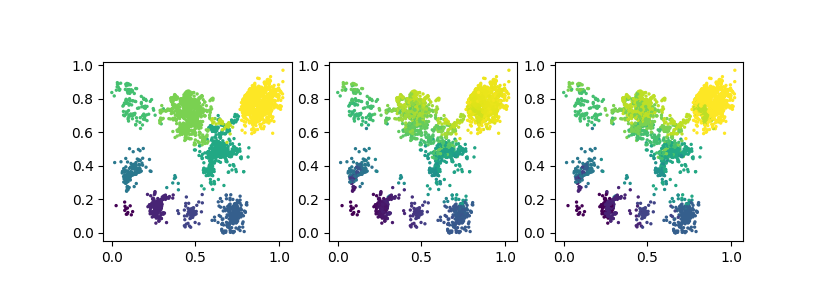
\includegraphics[width=\textwidth]{../images/example_prediction_2d.png}
}
\caption{\label{fig-example-prediction-2d}A top-down view of an example
prediction of the tree segmentation PointNet++ on a sample from the
validation dataset. \textbf{Left:} Points colored by label -- tree ID
within the patch. \textbf{Middle:} Points colored by the raw prediction
of the network (the regression head outputs a continuous prediction for
every point). \textbf{Right:} Points colored by the rounded prediction
-- converted from the continuous to the final integer tree ID.}
\end{figure}

\begin{figure}
\centering{
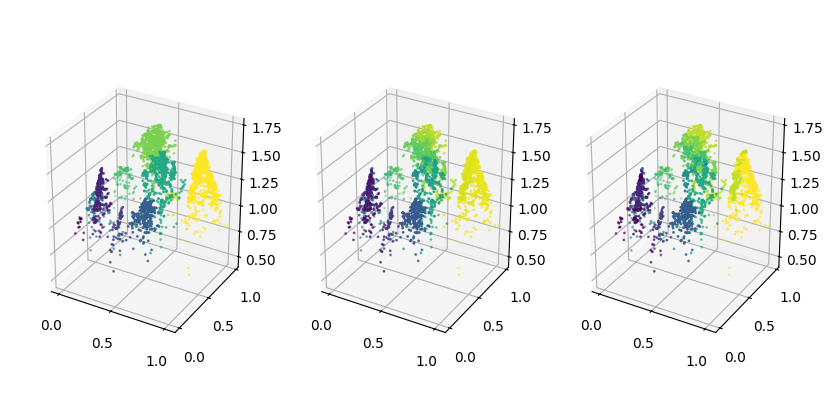
\includegraphics[width=\textwidth]{../images/example_prediction_3d.png}
}
\caption{\label{fig-example-prediction-3d}A 3D view of an example
prediction of the tree segmentation PointNet++ on a sample from the
validation dataset. \textbf{Left:} Points colored by label -- tree ID
within the patch. \textbf{Middle:} Points colored by the raw prediction
of the network (the regression head outputs a continuous prediction for
every point). \textbf{Right:} Points colored by the rounded prediction
-- converted from the continuous to the final integer tree ID.}
\end{figure}

Overall, the final model was selected less based on raw numbers such as maximum average validation accuracy or minimum average validation loss, but by expecting the visualizations of the predictions on a subset of samples from the validation dataset.

\section{Attribute prediction model training results}

To evaluate the performance of the attribute prediction models, 10-fold stratified cross validation was used, as well as a separate 40\% hold-out set.
For the tree species classification model, the stratification was performed using the labels directly.
For the diameter at breast height regression model, the stratification was performed on the label split into 5 equal-width buckets across the range.

\subsubsection{Tree species classification}

The tree species classification model was evaluated using accuracy and macro $F_1$-score (an average of $F_1$-scores across all the classes).
Figure~\ref{fig-cv-clf} shows out-of-fold metrics across all ten folds of cross-validation.
The average accuracy is 0.71, with a standard deviation of 0.06.
The average macro $F_1$-score is 0.70, with a standard deviation of 0.07.
The model is overall relatively consistent across all ten folds, showing that the cross-validation metrics estimates are reliable.

\begin{figure}
\centering{
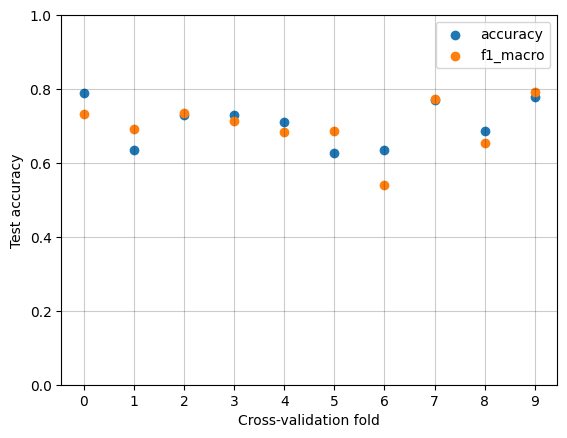
\includegraphics[width=\textwidth]{../images/train-tree-models-fig-cv-clf-output-1.png}
}
\caption{\label{fig-cv-clf}10-fold cross-validation results of the
species classification Random Forest model. The average accuracy is 0.71
with a standard deviation of 0.06. The average macro F-score is 0.70
with a standard deviation of 0.07. The model is overall stable across
all of the folds.}
\end{figure}

The holdout set was used to take a more in-depth look at the classification results.
Figure~\ref{fig-clf-confusion-matrix} shows the confusion matrix for the holdout set, with values normalized by row.
The set is relatively small – 158 examples, but enough to see some patterns emerge in the predictions.
The best overall species is spruce, and all coniferous species are better than all the deciduous species.
The model often confuses deciduous species, classifying alder as birch or tilia, aspen as birch, tilia as alder or birch.
This behavior is to be expected, as the shapes of deciduous species are very similar to each other and in complex in general.
The overall accuracy in the holdout set is 61\%.

\begin{figure}
\centering{
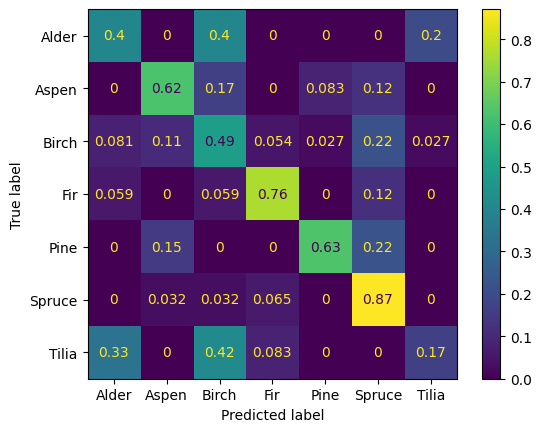
\includegraphics[width=\textwidth]{../images/train-tree-models-fig-clf-confusion-matrix-output-1.png}
}
\caption{\label{fig-clf-confusion-matrix}Confusion matrix for the tree
species classification Random Forest. Calulated on the 40\% holdout set
of 158 examples. Values normalized by row. The model confuses deciduous
species a lot more than coniferous ones.}
\end{figure}

\subsubsection{Diameter at breast height regression}

Diameter at breast height regression model was evaluated using root mean squared error (RMSE), mean absolute error (MAE), and coefficient of determination $R^2$.
The dataset here is smaller because diameter at breast height is only available for trees from the Lysva field inventory, while species are available for all trees in the individual tree point cloud dataset, some of which are from other surveys in the region.
Figure~\ref{fig-cv-reg} shows out-of-fold metrics across all ten folds of cross-validation.
Both the mean squared error and the mean absolute error are stable across the folds, with average RMSE 4.55 centimeters with a standard deviation of 0.19 and average MAE 3.49 centimeters with a standard deviation of 0.38.
Coefficient of determination $R^2$ is less stable.
Even though most folds have it around 0.6 to 0.8, there are two folds where it drops to below 0.2 and even close to 0, meaning that the model there is no better than predicting the mean dbh for every input.
This drops the average $R^2$ to 0.53 with a standard deviation of 0.24.

\begin{figure}
\centering{
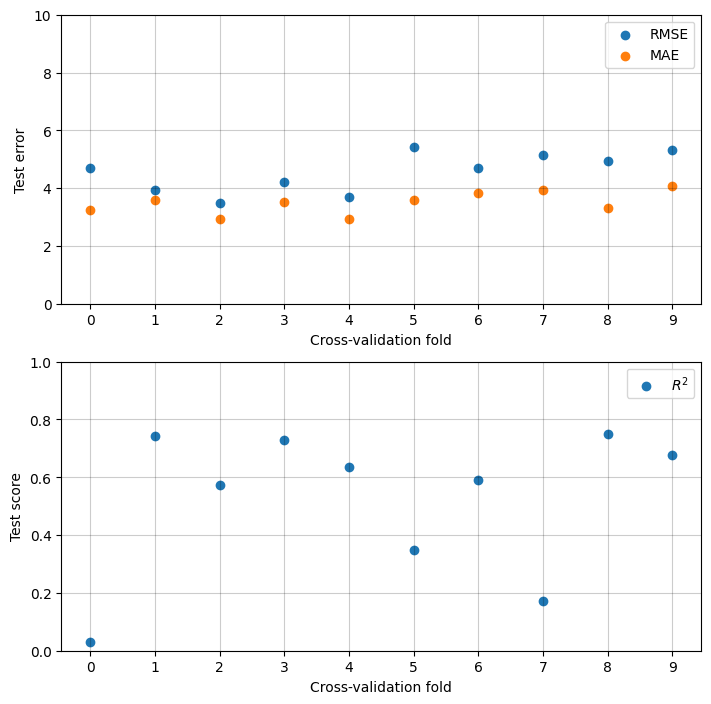
\includegraphics[width=\textwidth]{../images/train-tree-models-fig-cv-reg-output-1.png}
}
\caption{\label{fig-cv-reg}10-fold cross-validation results of the dbh
regression Random Forest model. The average RMSE is 4.55 centimeters
with a standard deviation of 0.19. The average MAE is 3.49 centimeters
with a standard deviation of 0.38. The average coefficient of
determination \(R^2\) is 0.53 with a standard deviation of 0.24. The
model is relatively stable in terms of the errors, but the coefficient
of determination is all over the place.}
\end{figure}

Similar to the classification model, the holdout set was used to take a more in-depth look at the regression results.
Here the holdout set is even smaller than for regression – 68 samples.
Figure~\ref{fig-reg-residuals} offers a collection of diagnostic visualizations aimed to help better understand the regression performance.
On the top left is the residual plot, where the differences between the actual dbh and the predicted dbh are plotted against the actual dbh values.
Ideally, the points should be around a horizontal line at zero, shown in black, without any patterns.
This would mean that the size of the error does not depend on the value of dbh.
The resulting dbh regression model shows a trend, which means it tends to overestimate low dbh values and underestimate high dbh values.
A related plot is on the top right, showing the distribution of the residuals across the holdout set.
It should be centered around zero and as narrow as possible.
On the bottom left is a scatter plot of predicted dbh against the actual dbh.
Ideally, this should be a 45-degree line, shown in black.
Because of the underestimation on the high end and overestimation in the low end, the points seem to lie on a line with a smaller slope.
Although most points are in the middle, where the line is followed a lot more closely.
And, finally, a related plot on the bottom right, comparing distributions of the actual dbh and predicted dbh in the holdout set.
The same lack of extreme can be observed.

\begin{figure}
\centering{
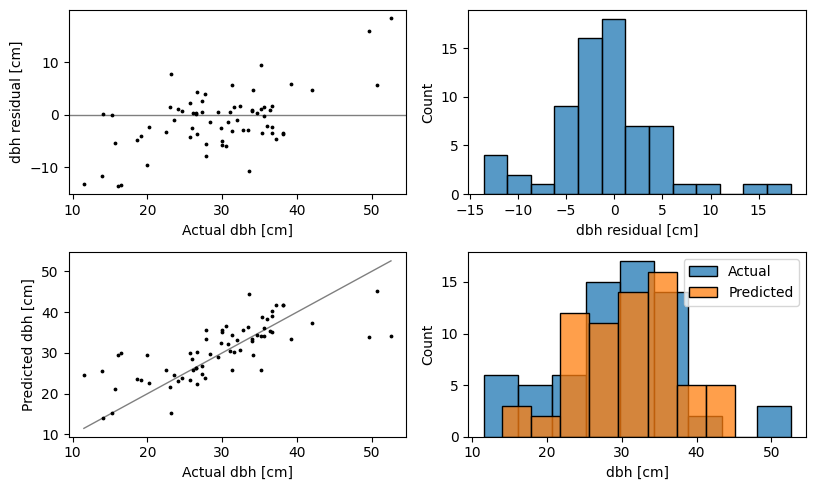
\includegraphics[width=\textwidth]{../images/train-tree-models-fig-reg-residuals-output-1.png}
}
\caption{\label{fig-reg-residuals}Quality assessment plots for the
diameter at breast height regression Random Forest. Calculated on a 40\%
holdout set of 68 examples. \textbf{Top Left:} Residual scatter plot:
difference between the prediction and the true value vs.~the true value.
Ideally the spread should be equal across the valu range. \textbf{Bottom
Left:} Predicted vs.~actual scatter plot. Ideally should be as close to
a line as possible. \textbf{Top right:} Distribution of the residuals.
\textbf{Bottom right:} Distribution of the predicted and actual values
of dbh.}
\end{figure}

\section{Validation on the Lysva field inventory data}

To validate the framework, the results were evaluated on the Lysva field inventory dataset, described in Section~\ref{sec-lysva-dataset}.
The mean X and Y coordinates of each segmented tree were calculated to convert the cloud into a set of points, where each point represents a candidate detected tree.
The maximum height of the points in the cluster was used as the height of the detected tree.
Then the algorithm described in Section~\ref{sec-matching-algorithm} was applied to match the detected trees their corresponding the ground truth trees, if any.
The matching algorithm was run with max distance of 5 meter and max height difference of 3 meters (ignored for ground truth trees that don't have measured height).
Then, precision, recall, and $F_1$-score were calculated for the detection results, and for the true positive matches the average distance between the detected tree and the actual tree, species classification accuracy and macro $F_1$-score, and diameter at breast height errors are calculated.

Table~\ref{tbl-detection-results} shows the tree detection metrics.
When interpreting the metrics, the reader is advised to keep in mind the limitations of the distance metric mentioned in @sec-matching-algorithm, and instead focus on the $F_1$-score as the most informative metric.
The overall average $F_1$-score for tree detection by the described system is 0.63.

\begin{table}
    \centering
    \caption{Results of the tree detection across all plots in the Lysva field survey.}
    \label{tbl-detection-results}
    \begin{tabular}{lrlrrrrr}
    \toprule
     & Tree count & Dominant type & Point density & Recall & Precision & F1-score & Distance \\
    Plot &  &  &  &  &  &  & \\
    \midrule
    1 & 420 & Deciduous & 31.7 & 0.83 & 0.63 & 0.72 & 0.77 \\
    2 & 365 & Deciduous & 47.9 & 0.61 & 0.72 & 0.66 & 0.81 \\
    3 & 332 & Deciduous & 40.3 & 0.63 & 0.49 & 0.56 & 0.85 \\
   4 & 261 & Coniferous & 33.5 & 0.85 & 0.50 & 0.63 & 1.06 \\
   5 & 208 & Coniferous & 14.2 & 0.68 & 0.55 & 0.61 & 0.97 \\
   6 & 290 & Coniferous & 39.1 & 0.80 & 0.52 & 0.63 & 0.83 \\
    7 & 408 & Deciduous & 41.9 & 0.65 & 0.62 & 0.63 & 0.85 \\
   8 & 341 & Coniferous & 35.5 & 0.87 & 0.57 & 0.69 & 0.93 \\
   9 & 459 & Coniferous & 42.1 & 0.56 & 0.65 & 0.60 & 0.92 \\
   10 & 518 & Deciduous & 42.9 & 0.42 & 0.92 & 0.58 & 0.99 \\
    \midrule
    & & & Average: & 0.69 & 0.62 & 0.63 & 0.90 \\
    \bottomrule
    \end{tabular}
\end{table}

Figure~\ref{fig-lysva-confusion-matrix} shows the confusion matrix for species prediction calculated for true positive matches.
Note that willow trees are not included, as the model has not seen any in the training data, and all pine predictions are counted as spruce instead.
The pattern of the confusion matrix is similar to the evaluation on the holdout set.
The overall accuracy is 66.1\%.
The overall macro $F_1$-score is 55.4\%.

\begin{figure}
\centering{
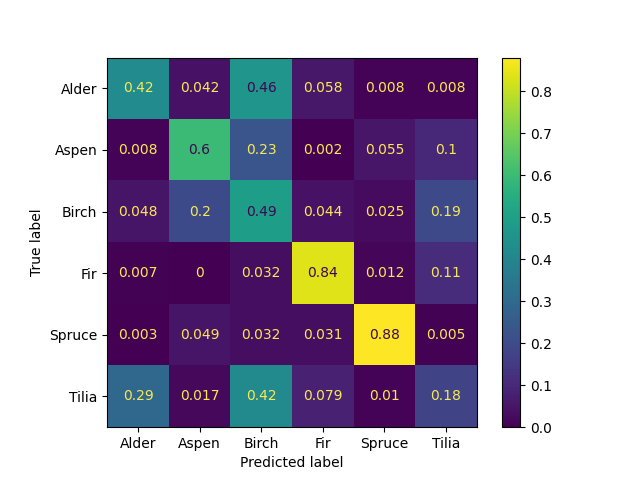
\includegraphics[width=\textwidth]{../images/lysva-confusion-matrix.png}
}
\caption{\label{fig-lysva-confusion-matrix}Confusion matrix for the tree
species classification on true positive detected trees in the Lysva
field inventory plots.}
\end{figure}

Figure~\ref{fig-lysva-regression-metrics} show the quality assessment plots for the results of diameter at breast height regression.
It's obvious from the plots that the individual tree dataset is not representative of the entire Lysva dataset in terms of dbh, as the range of dbh in there is not wide enough.
The distributions show that the individual trees dataset has higher mean dbh values than the overall distribution, which makes the model eager to overestimate a lot.
This effect is no doubt connected to the sampling bias mentioned in the description of the individual trees dataset: trees were selected by humans based on how easy they are to extract from a large point cloud.
As the result, the predictions outside the range seen by the Random Forest are constant.
Within the covered range, however, the behavior is similar to what was observed on the holdout set: a trend in the residual plot indicating over- and underestimation of low and high values, and errors close to zero near the middle of the range.
The overall root mean squared error is 5.37 centimeters.
The overall mean absolute error is 4.21 centimeters.
The overall coefficient of determination $R^2$ is 0.65.

\begin{figure}
\centering{
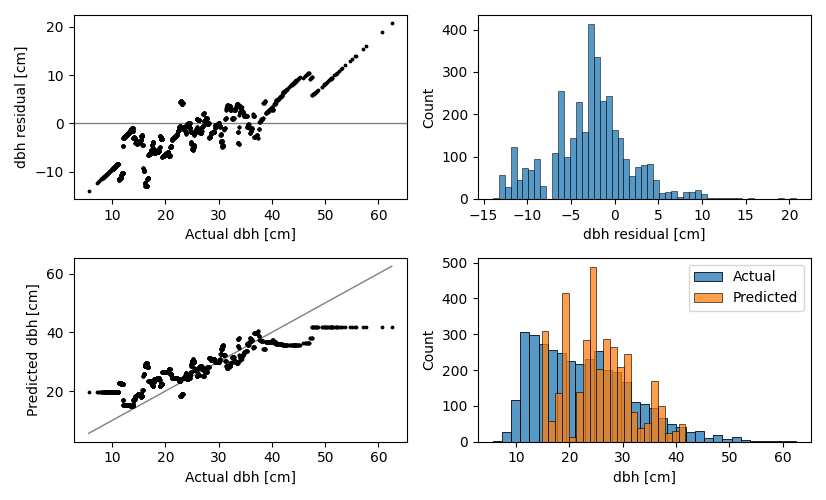
\includegraphics[width=\textwidth]{../images/lysva-regression-metrics.png}
}
\caption{\label{fig-lysva-regression-metrics}Regression quality
assessment plots plots for the diameter at breast height regression on
true positive detected trees in the Lysva field inventory plots.}
\end{figure}
\chapter{Conclusion}\label{cap:conclusion}

\epigraphhead[50]{%
    \epigraph{"A PhD research project is an academic exercise of given effort and length." }{Dr. Ron Anderson, PhD adviser of prof. Clement Fortin}
}

This thesis is dedicated to designing, implementing, and testing of a framework for estimating forest parameters at the scale of individual trees.
The proposed framework relies on fusion of UAV LiDAR point clouds and RGB orthophotos data, deep neural networks designed for processing 3D points clouds to segment the data into individual trees, and a collection of parameter-specific classic machine learning models to process the segmented trees and predict forest parameters of interest.
An end-to-end implementation is described in detail, with parts of the system evaluated separately, and the overall system validated on a detailed manual field inventory dataset.
The main contributions of this thesis are thus the design, implementation, and experimental verification of said framework.
Moreover, during the work on the thesis, both original datasets used for training the models were published into open access, to hopefully be useful to the research community with a rapidly growing interest in detailed digital forest inventories \citep{dubrovinExplorationPropertiesPoint2024, dubrovinOpenDatasetIndividual2024}.
I believe the release of data into open access is worthy of including as a contribution, especially in the current era of commercial machine learning\footnote{I am purposefully avoiding the term "artificial intelligence" as it seems to have been abused so much as to become practically meaningless, and thus not useful in technical context.}.
When having good data is an advantage, less people are willing to make their data public, which makes it harder for researchers to explore, develop, and compare novel approaches.

Coming back to the research question and the hypothesis stated in Section~\ref{sec-research-question}, I want to address the ways I believe the proposed framework answers it.
As already mentioned there, the baselines are the manual forest inventory and the widely used area-based approach described in Section~\ref{sec-area-based-approach}.
The cost reduction mainly comes from the choice of the platform for remote sensing observations.
Using UAVs is cheaper than purchasing high resolution data from satellites or planes, and it offers a lot more control over the acquisition parameters, although it requires trained operators.
The effort reduction mainly comes from dramatic decrease in the amount of required field inventory data, which is very labor-intensive to collect.
UAVs are also allow to cover huge areas easily by a few people, unlike fully manual inventories or those based on terrestrial LiDAR measurements, where a forester or an operator needs to cover the entire area of interest by foot.

The reported experimental results achieved by the implemented system are by no means state of the art, but they do serve as a proof of concept.
The current state of the system, described in the previous chapter, can be seen as a baseline, since it prioritizes simple components to show that the overall system has potential.
And I believe the resulting framework has potential, with specific steps I would try if I had unlimited time, listed in the next section.

\section{Potential further improvements}

I see numerous ways to potentially improve the results of the proposed system.
Some of the most important are as follows:

\begin{itemize}
\item Use of more advanced tree segmentation network architectures.
  As mentioned, the PointNet++ is a pioneering model in the field of deep learning on 3D point clouds that was chosen because it is relatively easy to implement and work with.
  It is still competitive in many tasks, but the field of deep learning is evolving rapidly, and many more powerful architectures were suggested and proven since its release.
  The framework will definitely benefit from a better, more efficient tree segmentation network.
\item Use of more advanced feature extraction for RGB orthophoto-based features.
  For the same reason the PointNet++ was chosen as a baseline for tree segmentation, a very basic approach was used to extract features from RGB orthophotos.
  Despite being better than just RGB colors, these features still offer very limited representation power.
  Instead, convolutional neural networks specialized in creating good representations for downstream tasks can be used.
\item Use of open-access datasets for pretraining.
  At its current state, the tree segmentation network learns to perform a very hard task from scratch on a dataset of a very limited size.
  I believe it can benefit from first training on similar, but larger dataset, for example, the NeonTreeEvaluation Benchmark \citep{weinsteinDataNeonTreeEvaluationBenchmark2022}.
  It is briefly described in the comparison subsection of the Lysva field inventory section.
  The bounding boxes from the orthophoto can be used to label the point cloud for tree segmentation.
  The labels will be noisy, but pretraining on a large amount of noisy data often shows good results.
\item Use of more sophisticated techniques for creating synthetic forest patches.
  Both the sampling of the trees and the placement onto the patch can be improved.
  For example, sampling can take into consideration the species of the trees, to make the patches more realistic: some fully coniferous, some fully deciduous, some mixed.
  Placing of the trees can use packing algorithms, or try to mimic the spatial distribution of trees in the inventory.
\item Use of more sophisticated augmentations to make the synthetic forest patches look as close as possible to real forest patches.
  For example, the height-depended dropout can be improved to take into account canopy density and overlap.
  A shorter tree almost completely covered from above by a larger tree should have fewer points overall, not just at low heights relative to its highest point.
\item Use of a more careful approach to training attribute prediction models.
The results of the second step can be further improved by adopting a more careful approach to modeling, including a more careful approach to feature engineering and model selection.

\end{itemize}


\newacronym{sk}{SK}{Skolkovo Institute of Science and Technology}
\newacronym{sysml}{SysML}{Systems Modeling Language}

\begin{singlespace}
\printglossary
\end{singlespace}

\phantomsection 
\addcontentsline{toc}{chapter}{Bibliography} 
%% This defines the bibliography file (main.bib) and the bibliography style.
%% If you want to create a bibliography file by hand, change the contents of
%% this file to a `thebibliography' environment.  For more information 
%% see section 4.3 of the LaTeX manual.
\begin{singlespace}
\bibliographystyle{plainnat}
\bibliography{../references}
\end{singlespace}


%\appendix
%\chapter{Additional Resources}
\label{sec:additional-resources}

\Autoref{tab:comparison_x_and_y} contains some additional material.

\setlength{\tabcolsep}{0.5em} % for the horizontal padding
\renewcommand{\arraystretch}{2} % for the vertical padding
\begin{table}[ht!]
  \centering
  \begin{tabularx}{0.9\textwidth}{|p{8em}|p{6em}p{6em}X|}
    \hline
    \textbf{Feature}     & \textbf{Method X}      & \textbf{Method Y}                           & \textbf{References}                      \\
    \hline
    \rowcolor[HTML]{EFEFEF}
    Speed                     &  medium     &  slow          &       \citet{Skoltech2017}             \\
    \hline
    Cost                        & less            & more          &                                  \\
    \hline
    \rowcolor[HTML]{EFEFEF}
    Error                      &        2           &                   3                   &                                         \\
    \hline
  \end{tabularx}
    \caption{Comparison of X and Y}
    \label{tab:comparison_x_and_y}%
\end{table}

\end{document}

